\documentclass[runningheads]{llncs}

\usepackage{tikz,mathpartir}
\usepackage{mathtools}
\usepackage{amsmath,amssymb,mathabx}
%\usepackage{unicode-math}
\usepackage{tikz}
\usetikzlibrary{external}
\usepackage{hyperref}
\usepackage{nccrules}


\AtBeginDocument{\renewcommand\setminus{\smallsetminus}}

\DeclareMathOperator{\dom}{dom}

\newcommand{\symb}[1]{\makebox{\it #1}}
\newcommand{\dbllbrack}{\{\hspace{-0.88ex}\{}
\newcommand{\dblrbrack}{\}\hspace{-0.87ex}\}}

\newcommand\mpar[1]{{\left(#1\right)}}
\newcommand\mbrk[1]{{\left[#1\right]}}
\newcommand\mbrc[1]{{\left\{#1\right\}}}
\newcommand\mdbrk[1]{\left\ldbrack#1\right\rdbrack}
\newcommand\card[1]{{\left|#1\right|}}
\newcommand\psubst[1]{\mbrc{\!\!\mbrc{#1}\!\!}}
\newcommand\subst[2]{\mbrk{#1\middle/#2}}
\newcommand\midbar{\,\middle|\,}
\newcommand\mset[2]{\mbrc{#1\midbar #2}}

\newcommand\act{\mathrm}
%\newcommand\OTbase[4]{\text{\small\(%
%	\setlength\arraycolsep{2pt}\everymath{\displaystyle}%
%	\renewcommand\arraystretch{1}%
%	\begin{array}{c}%
%	#2,#3,#4 \\\noalign{\color{red}\hrule\vspace{1pt}\hrule}
%	#1
%	\end{array}\)}}
\newcommand\OTbase[4]{\text{\small\(%
	\setlength\arraycolsep{2pt}\everymath{\displaystyle}%
	\renewcommand\arraystretch{1}%
	\begin{array}{c}%
	#2,#3,#4 \\\noalign{\color{red}\hrule}
	#1
	\end{array}\)}}

\newcommand\OThelperdonotuse[2][\top]{\OTtemporary{#1}{\mbrc{#2}}}
\newcommand\OTd[2]{\newcommand\OTtemporary{\OTbase{#1}{\mbrc{#2}}}\OThelperdonotuse}

\newcommand\OT[3]{\OTbase{#1\xrightarrow{\raisebox{-1.5pt}[.8\height][0pt]{\makebox[1.4\width]{\(\scriptstyle #3\)}}}#2}}
\newcommand\OTx[4]{\OT{s_{#1}}{s'_{#1 #2}}{\alpha_{#1 #2}}{\beta_{#3 j}^{j \in J'_{#4}}}{g_{#1 #2}}{\psi_{#1 #2}}}
\newcommand\OTg{\OTx{}{}{}{}}

\theoremstyle{plain}
\newtheorem{thm}{Theorem}
\newtheorem{lem}{Lemma}
\newtheorem{cor}{Corollary}
\newtheorem{prop}{Proposition}

\theoremstyle{definition}
\newtheorem{defi}{Definition}
\newtheorem{exi}{Example}

\newcommand\comment[3]{\colorbox{#1}{#2}\marginpar{#3}}
\newcommand\Rabea{\comment{yellow}}
\newcommand\Ludo{\comment{green}}
\newcommand\Eric{\comment{cyan}}
\newcommand\Quentin{\comment{pink}}

\newcommand\nmm[1]{\(\displaystyle #1\)} % nmm for Nice Math Mode
\newcommand\hyp[1]{\TextOrMath{(H#1)}{\tag{H#1}}}
\newcommand\goal[1]{\TextOrMath{(G#1)}{\tag{G#1}}}
\newcommand\defitem{\item[\bullet]}

\newcommand\setR{\mathbb{R}}
\newcommand\setZ{\mathbb{Z}}
\newcommand\setN{\mathbb{N}}

\newcommand\choice[1]{\left\{\everymath{\displaystyle}%
	\begin{array}{lr}#1\end{array}\right.}
\newcommand\subbox[1]{{\makebox[.5\width]{\(\scriptstyle #1\)}}}
\newcommand\bigsymb[2][\Large]{\text{#1\nmm{#2}}} % DeclareMathDelimiter?
\newcommand\defnotation{\text{ defined as }}
\newcommand\defobject{\DOTSB\;{\coloneq}\;}
\newcommand\nwedge{\DOTSB\;{\wedge}\;} % when you want to force space
\newcommand\qwedge{\DOTSB\quad{\wedge}\quad}
\newcommand\wrel[4][]{#2 \overset{#1}\leq_{#4} #3}
\newcommand\fvars[1]{\mathit{vars}\mpar{#1}}
\newcommand\fguard[1]{\mathit{guard}\mpar{#1}}
\newcommand\fOT[1]{\mathrm{OT}\mpar{#1}}
\newcommand\terms{{\mathcal{T}}}
\newcommand\formulae{{\mathcal{F}}}
\newcommand\actions{{\mathbb{A}}}
\newcommand\rver[3][\!\!]{#2_{#1#3}}
\newcommand\rterms[1][\emptyset]{\rver{\terms}{#1}}
\newcommand\rformulae[1][\emptyset]{\rver{\formulae}{#1}}
\newcommand\ractions[1][\emptyset]{\rver[]{\actions}{#1}}
\newcommand\values{\mathcal{P}}
\newcommand\labels{\mathcal{A}}
\newcommand\reach[1]{\checkmark_{\!\! #1}}

\tikzstyle{every edge} = [draw,-latex,every node/.style={auto}]
\tikzstyle{state} = [draw,circle,minimum size=1cm,inner sep=1mm]
\tikzstyle{initial} = [double,double distance=1mm,minimum size=.95cm,inner sep=.5mm,outer sep=.5mm]
\tikzstyle{init} = [double,double distance=1.5pt,edge label=\(\mbrc{#1}\)]
\tikzstyle{dir} = [out=#1+15,in=#1-15,looseness=10]


\begin{document}
%
\title{Refinements for open automata}
%
%\titlerunning{Abbreviated paper title}
% If the paper title is too long for the running head, you can set
% an abbreviated paper title here
%
\author{
Rabéa\inst{1}\orcidID{1111-2222-3333-4444} \and
Quentin\inst{1,2}\orcidID{1111-2222-3333-4444} \and
Ludo\inst{2}\orcidID{0000-1111-2222-3333} \and
Eric\inst{3}\orcidID{2222--3333-4444-5555}}
%
\authorrunning{Rab\'ea Ameur-Boulifa et al.}
% First names are abbreviated in the running head.
% If there are more than two authors, 'et al.' is used.
%
\institute{blabla
\email{lncs@fff}\\
\url{http://www.springer.com/gp/computer-science/lncs} \and
blibli\\
\email{\{abc,def\}@fff}}
%
\maketitle              % typeset the header of the contribution
%
\begin{abstract}
\TODO{ The abstract should briefly summarize the contents of the paper in 150--250 words.}

Establishing equivalences and refinement relations between programs is an important mean for 
verifying the correctness of programs, by formally proving the relation between a specification and an implementation, 
proving that two implementation are equivalent, or justifying optimisations and transformations, by establishing that the
behaviours of a modified program simulate those of to the source one.

In this article, we discuss a notion of refinement between so-called "open automata", which are symbolic
behavioural models for communicating systems. Open automata may have "holes" modelling elements of their
context, and can be composed by instantiation of the holes. This allows for a compositional approach for
verification of their behaviour, essential to address proofs about large realistic systems.

We define several variants of refinement between systems including either equal or different sets of holes, and 
show under which conditions these refinements are preserved by composition of open automata. We also discuss
the relations between these refinements and the existence of deadlocks.
We illustrate these notions on several simple use-cases.


\keywords{Labelled transition systems  \and Refinement \and Composition.}
\end{abstract}
%
%
%
\section{Introduction}
\TODO{1.5 pages}



Contributions:

We first: introduce open automata (NOT NEW), their composition, 
and the deadlock-free composition.

Then we define a refinement relation for open automata that has the following characteristics:

- good behaviour wrt composition

- refinement does not introduce deadlock

- a first relation that focuses on the automaton part 
and a second that deals with open behaviour

we will see that having at the same time composition and transitivity also raises challenges; we introduce a new form of refinement relation that addresses this challenge.


\section{Related Work}
\label{sec:sota}

\TODO{1 page}


The notion of refinement aims captures the relation between  a specification and an implementation of the same component. It is usually defined as trace inclusion or simulation \cite{Milner:1980, Kouchnarenko:2007}; this ensures that all behaviours of the implementation must be also behaviours of the specification. This definition, which is based on systems whose behaviour is fully defined, is not well-suited for open systems,  as it requires to reason also about unspecified behaviours.

There are some works that have focused on  the refinement of open systems. Defining refinement of open systems as trace inclusion  is  addressed  as a notion of subtyping in type theory 
\cite{GayH:2005,BravettiZ:2021}. Such refinement is  instead based  on interface-oriented approach, it allows the expression more internal choices and less external choices. The refinement of open systems is also defined in terms of  alternating simulation \cite{Alur:1998,deAlfaro:2021}, which deals with game-based models.
Alternating simulation that is originating from the game theory \cite{deAlfaro:2003} allows  the study of relation between individual components by viewing them as alternating transition systems. In particular,  a refinement of game-based automata expresses that the refined component can offer more services (input actions) and fewer service demands (output actions). However, the composition of such automata may
lead to illegal states, where one automaton issues an output that is not acceptable as input in the other one. The theory of alternating simulation provides an optimistic approach to compute compatibility between automata based on the fact that each automaton expects the other to provide  legal inputs, i.e, two components can be composed if there is an environment where they can work together. As we shall see in this paper, 
our approach to design refinement  has some commonalities with that of the above mentioned \cite{deAlfaro:2021}: both are process-oriented approach even if they are not based on the same notion of simulation and they are based on optimistic approach to composition. 
For the composability, we shall see that we use the notion of comparability of holes (similar to the notion of compatibility), which is explicitly encompassed in the definition of composition.

 



Previous work on open automata focused on equivalence relations compatible with composition.
In an article by Hou, Zechen and Madelaine \cite{10.1145/3372884.3373161}, a computable bisimulation is introduced and proved equivalent to the previous bisimulation already introduced.
In a more recent work by Ameur-Boulifa, Henrio and Madelaine \cite{2007.10770}, a weak version of the bisimulation on open automata is introduced.
These works differ from ours because the relation introduced in this report is a refinement relation in the form of a simulation and not a bisimulation.
Also we do not have results as strong as computability neither a weak version able to tackle silent actions.

\TODO{Some related work on other models than open automata introduce refinement relations.
In a chapter by Bellegarde, Julliand and Kouchnarenko \cite{10.1007/3-540-46428-X_19}, a simulation relation on transition systems is introduced.
This simulation encompass action refinement, is able to deal with silent actions and is compatible with parallel composition.
Here the refinement relation does not consider action refinement as valid but it should be done in future work.
Also they check how LTL properties are preserved or combined using their refinement which we do not do.
However their model is less expressive: the transition system model is less expressive than open automata and the parallel composition is less expressive than composition on open automata.
In a later report by Kouchnarenko and Lanoix \cite{10.1007/978-3-540-70881-0_26}, the refinement relation they introduce is on LTS (labelled transition systems).
Their relation additionally prevents deadlock and livelocks.
The composition is also extended to synchronised composition which is more expressive.
In our work we also deal with deadlocks but not with livelocks since the latter arise only with silent actions.
This work is closer than the previous one to what we do here, still open automata are more expressive than LTS and composition is more general than synchronised composition.}

A refinement relation on models nearer to open automata is introduced in an article by Zhang, Meng and Lo \cite{Zhang2014}.
In their article they work with transition systems with variable which makes the state space potentially infinite.
This aspect is also present in open automata.
They show how invariants, a notion near to our reachability predicates, are composed.
By relation on these invariants they introduce several refinement relations.
We could have done something similar for non-blocking composition reachability predicates which are introduced in Section \ref{sec:proofelts}.

On the deadlock prevention aspect, an article by Dihego, Sampaio and Oliveira \cite{DIHEGO2020110598} present a refinement relation on process algebra (translated to LTS).
This refinement relation is a special case of inheritance and prevents the introduction of deadlocks.
Their refinement and inheritance are quite the opposite of our refinement in terms of new behaviours.
They have channels, interfaces, inputs and outputs, which in the open automata model can be compared to action labels, holes and action data for both inputs and outputs.
They have a rich composition as open automata but the introduction of deadlock is already prevented by a well chosen set of composing operations.
Also their composition is slightly different than the one on open automata because they can cause loops by linking two channels of the same process, where in open automata the composition makes an oriented tree.
In their model there is an explicit deadlock and a successful termination where in open automata there are no explicit termination.
We define a deadlock as a configuration without possible transition and assume what is a deadlock when comparing the open automata.
To define their refinement and inheritance relation they use trace and failure semantics, which are weaker than (bi)simulations \cite{10.5555/640428.640430} and could break with open automata composition.


\section{Background: Open Automata and their Composition}\label{sec:background}
\TODO{3.5 pages}

This section presents our notations and the principles of automata. Except for minor changes in the notations, compared to previous works~\cite{pnets} the only new contribution is the definition of a composition operator for open automata.
%
%Notations will be defined with the operator \(\defnotation\) and names are given with the operator \(\defobject\) as follows:
%\begin{align*}
%	\mathit{notation\_with\_variables} & \defnotation \mathit{notated\_object\_using\_the\_variables} \\
%	\mathit{name} & \defobject \mathit{fully\_defined\_mathematical\_object}
%\end{align*}

%Throughout this paper, tuples will be noted differently depending on what they represent.
%This helps distinguishing the manipulated objects.
%Every such notation will be introduced in the definition of the object.

Families of values, or equivalently maps will be noted \(\mset{i \mapsto x_i}{i \in I}\), \(\mset{i \gets x_i}{i \in I}\) or \(x_i^{i \in I}\). % TODO: introduire le fait que \exists c_j^{j \in J} défini J et {j \mapsto c_j}
%For instance \(\mpar{ax}^{x \in \setR}\) represents a scaling function, \(c^{i \in I}\) is a constant function over \(I\).
%They will be used depending on what is more convenient.
%For instance \(\mbrc{\alpha \mapsto 1, \beta \mapsto 2, \gamma \mapsto 3}\) has no simple generating expression and is better represented with the finite version of first notation.
The disjoint union on set is noted \(\uplus\)\footnote{\(\uplus\) notation either supposes that the sets are disjoint or rename conflicting objects depending on the context}. Disjoint union is also used on maps.
%There are several ways of ensuring a union is disjoint, we will indifferently either suppose sets are disjoint or rename conflicting object (useful for variables).
%The disjoint union of two maps \(\varphi: I \to X\) and \(\psi: J \to Y\) with \(I \cap J = \emptyset\) is noted \(\varphi \uplus \psi\) and has the following signature \(I \uplus J \to X \cup Y\).
In a formula, a quantifier followed by a finite set will be used as a shorthand for the quantification on every variable in the set:
\(\forall \mbrc{a_1, \dots, a_n}, \exists \mbrc{b_1, \dots, b_m}, P\) means \(\forall a_1, \dots, \forall a_n, \exists b_1, \dots, \exists b_m, P\).

%\begin{definition}[Expression algebra, Action algebra, Formulas, Terms]
An expression algebra \(E\) is the disjoint union  of  terms,  actions, and  formulas
\( E=\terms \uplus \actions \uplus \formulas\) .
\(\terms\) and \(\actions\) are term algebras \TODO{do we explain term algebras}.
The formulas \(\formulas\) contain at least first order formulas and equality\footnote{Equality does not need to be only syntactic.} over \(\terms\) and \(\actions\). 
%\end{definition}

 \(\fvars{e}\) is the set of variables in \(e \in E\) that are not bound by any binder. An expression is closed if \(\fvars{e}=\emptyset\).
The set \(\values\) denote values which is a subset of closed terms. \(\rformulas[V]\) is the set of formulas $f$ that only use variables in $V$, i.e. the formulas such that  \(\fvars{f}\subseteq V\).

The substitution in \(e \in E\) of \(x \in \fvars{e}\) by \(t \in \terms\), is denoted \(e\subst{t}{x}\), and its generalisation to the parallel substitution of variables in \(V\) by \(\psi: V \to \terms\) is denoted \(e\psubst{\psi}\).


 We suppose given a decidable satisfiability relation on formulas, \({\vdash} f\) is the satisfiability over closed formulas.
% In practice one of our objective is to be able to use a SMT solver to reason automatically on the properties of open automata, in this case
%\(\vdash\) can hence be interpreted as an indicator of what is given to the SMT; it separates the external logic and the logic on \(\formulas\).
We will  use two satisfiability relations:
\begin{itemize}
\item The satisfiability of a formula \(f \in \formulas\) under some valuation \(\sigma: V \to \values\) is defined as follows:
\( \sigma \vdash f \iff \vdash \exists \fvars{f\psubst{\sigma}}, f\psubst{\sigma} \)
\item The satisfiability of a formula \(f \in \formulas\) with some variable set \(V\) as context is defined as follows:
\( V \vdash f \iff  \vdash \forall V, \exists\mpar{\fvars{f} \setminus V}, f \)
\end{itemize}

%For instance a formula with quantifiers on variables might not be provable even if it is true for all values of these variables.

\subsection{Open Automata}\label{sec:def}
 Open automata (abbreviated OA) are labelled transition systems with variables  that can be used to compose other automata: they are made of transitions that are dependent of the actions of ``holes'', a composition operation consists in filling a hole with another automaton to obtain a more complete automaton. The variables makes the OA symbolic, and the holes allow for a partial definition of the behaviour.

\begin{definition}[Open transition, Open automaton (OA)]
An \emph{open automaton} is a tuple \(\OAg\) with \(S\) the set of states, \(s_0 \in S\) the initial state, \(V\) the finite set of variable names, \(\sigma_0: V' \to \values\) the initial valuation of variables where \(V' \subseteq V\), \(J\) the set of hole names and \(T\) the set of open transitions. 

An \emph{open transition} is a tuple \nmm{\OTg} with \(s, s' \in S\) the source and target states, \(\alpha \in \actions\) the produced action, \(J' \subseteq J\) the holes involved in the transition, \(\beta_j \in \actions\) the actions of the holes, \(g \in \formulas\) the guard and \(\psi: V \to \terms\) the variable assignments.
To be well-formed, an open transition should use only variables of the automaton and variables appearing in the involved actions, formally: 
\begin{align*}
\fvars{g}&\subseteq \fvars{\alpha}\cup \bigcup_{j \in J'} \fvars{\beta_j} \cup V \\ \forall v\in V.\, \fvars{\psi(v)}&\subseteq \fvars{\alpha}\cup \bigcup_{j \in J'} \fvars{\beta_j} \cup V
\end{align*}
\end{definition}





%\TODO{useful or not?}
\begin{definition}[Guard, Out-transition, Transition variables]
Let \(V\) be the variable names of the considered automaton, \(T\) its transitions and \(r\) one of its states.
\(\fOT[T]{r} \in T\) are called the out-transitions of the state \(r\).
\(\fIT[T]{r} \in T\) are called the in-transitions of the state \(r\).
When the transition set is clear from the context, it will be omitted.
The local variables of a transition \(\fvars{t}\) are all variables appearing in transition \(t\) except the global variables of the automaton.
\begin{align*}
	\fOT[T]{r} & = \mset{\OTg \in T}{s = r} &
	\fIT[T]{r} & = \mset{\OTg \in T}{s' = r} \\
\end{align*}
\vspace{-1cm}
\begin{mathpar}
	\fguard{\OTg} \!=\! g \qquad
	\fvars{\OTg} \!=\! \mpar{\fvars{\alpha}  \cup \bigcup_{j \in J'} \!\fvars{\beta_j} } \setminus V
\end{mathpar}
\end{definition}


The following terminology will be used to reason on open automata
\begin{definition}[Configuration, instantiated transition]
A pair consisting of a state and a valuation is called a \emph{configuration}.
An \emph{instantiated transition} of an automaton \(\OAg\) is a transition  \(t\psi\) where $t\in T$ and $\psi$ is a  well-formed substitution with $\dom(\psi)=vars(t)$. %\setminus V$.
\end{definition}

\paragraph{Open automaton composition}

Open automata are partially specified automata, that partiality comes mostly from the holes.
A hole is an interface in which we can plug an open automaton.
The plugging operation is called composition.
The composition of open automata was already implicitly defined by the means of composition on pNets in previous work \cite{henrio:01299562} but never completely formalised on open automata.
The definition of composition below is a direct translation of what happens with pNets composition without the need of introducing pNets.

\TODO{peut etre echanger c et p? ou c devient p et p devient? }
\begin{definition}[Composition of open automata] \label{Def:CompOA}
The composition of \(A_c = \OAg[c]\) in the hole \(k \in J_p\) of \(A_p = \OAg[p]\) is the OA defined as follows:
\[A_p\subst{A_c}{k} ::=  \OA{S_p \times S_c}{\mpar{s_{0p}, s_{0c}}}{V_p \uplus V_c}{\sigma_{0p} \uplus \sigma_{0c}}{J_c \uplus J_p \setminus \mbrc{k}}{T} \] \text{with }

\begin{align*}
T=& \mset{\OT{\mpar{s_p, s_c}}{\mpar{s'_p, s'_c}}{\alpha_p}{\beta_j^{j \in J'_c \uplus J'_p}}{g_p \wedge g_c \wedge \alpha_c = \beta_k}{\psi_p \uplus \psi_c}}{ \OT{s_p}{s'_p}{\alpha_p}{\beta_j^{j \in J'_p \uplus \mbrc{k} }}{g_p}{\psi_p} \in T_p, \OTx{c}{}{}{c} \in T_c} \\
	& \cup \mset{\OT{\mpar{s_p, s_c}}{\mpar{s'_p, s_c}}{\alpha_p}{\beta_j^{j \in J'_p}}{g_p}{\psi_p}}{\OTx{p}{}{}{p} \in T_p, k \notin J'_p, s_c \in S_c}
\end{align*}
\end{definition}
The first OA decides when the second can evolve by involving its hole in a transition:
The action emitted when \(A_c\) makes a transition is synchronised with the action of the hole \(k\) in transitions of \(A_p\) .

\paragraph{Relations between open automata}
A relation (bisimulation, refinement, etc.) between open automata requires to compare their states. To do so we will suppose that the variables of the two OAs are disjoint (a renaming of variables may have to be applied before comparing OA states)
\begin{definition}[Relation on OA states] Suppose $V_1$ and $V_2$ are disjoint.
A relation on states of \(\OAg[1]\) and \(\OAg[2]\) is a function \(R: S_1 \times S_2 \to \rformulas[V_1 \uplus V_2]\).
\end{definition}
The idea is that two states are related if the variables they refer to verify a certain formula. Additionally, we may check that initial states of the automata are related by checking that: \(\sigma_{01} \uplus \sigma_{022} \vdash R\mpar{s_{01}, s_{02}}\).

\TODO{I do not think we reason on configurations for the moment, if we want to, we should introduce this:}
Two configurations \(\mpar{s_1, \sigma_1} \in S_1 \times\mpar{V_1 \to \values}, \mpar{s_2, \sigma_2} \in S_2 \times \mpar{V_2 \to \values}\) are related iff \(\sigma_1 \uplus \sigma_2 \vdash R\mpar{s_1, s_2}\).

\paragraph{A bisimulation for open automata}

TODO OR NOT?

\subsection{Example}

As an example, the traffic light system  that controls  
 traffic at an intersection. The open automaton  
modeling this system  is illustrated in  Figure \ref{fig:tls}. This automaton has three states  remembering which coloured light
is on (Red, Yellow or Green). It includes two holes: a controller ($\symb{ctl}$) and a counter ($\symb{cnt}$)  depicting together the behaviour of the timer. The color switches when the counter and the controller component agree that the time is over. The new time limit can be set by the counter component and the exposed action to the environment is an unobservable  action $\tau$.

The open automata shown in Figure  \ref{fig:ctlandcnt} models  the timer. On the left, the controller component designed to be connected in the hole $\symb{ctl}$.  Its role is to decide the duration before switching the lights. 
We control the time interval for each light by setting them by prior knowledge:  17s for the first duration, 3s for the second, and 20s for the third. On the right, the tick counter component designed to be connected in the hole $\symb{cnt}$.                                                                                                                                     




In Figure \ref{fig:tlf} we present the composition of the three automata. Each state of the result of the composition consists  of  a state of traffic light system together with a state of controller component and one of counter component. The composed automaton  takes over  the same steps as the traffic light automaton but it also includes new steps,  indicting the change of states for the setting of timer. Its $\tau$ transitions involve both the traffic light automaton and the hole  automata, they correspond to  a joint step of  sending time thresholds of the controller, the time setting of the counter. For instance, the  $\tau$  transition starting from \(R1S\), it is obtained by composition of both 
\nmm{\OT{R}{R}{\tau}{\mbrc{cnt \mapsto \act{set}\mpar{x}, ctl \mapsto \theta\mpar{x}}}{\top}{\mbrc{}}}, \nmm{\OT{1}{2}{\theta\mpar{17}}{\mbrc{}}{\top}{\mbrc{}}} and   \nmm{\OT{S}{C}{\act{set}\mpar{x}}{\mbrc{}}{\top}{\mbrc{t \gets x, c \gets 0}}}. \\ 
However, the joint composition of transitions  \nmm{\OT{R}{R}{\tau}{\mbrc{cnt \mapsto \act{set}\mpar{x}, ctl \mapsto \theta\mpar{x}}}{\top}{\mbrc{}}}, \nmm{\OT{2}{3}{\delta\mpar{x}}{\mbrc{}}{\top}{\mbrc{}}} and 
\nmm{\OT{C}{C}{\act{tick}}{\mbrc{}}{c < t}{\mbrc{c \gets c + 1}}} is not agreed because it would produce a transition whose guard is not satisfiable. It will produce the following transition: \nmm{\OT{R2C}{R3C}{\tau}{\mbrc{}}{\top \wedge \top \wedge c < t \wedge \act{set}\mpar{x} = \act{tick} \wedge \theta\mpar{x} = \delta\mpar{x}}{\mbrc{c \gets c + 1}}} which requires to be triggered  the equality of completely different actions. 








\begin{figure}[!tb]
\centering
\scalebox{.75}{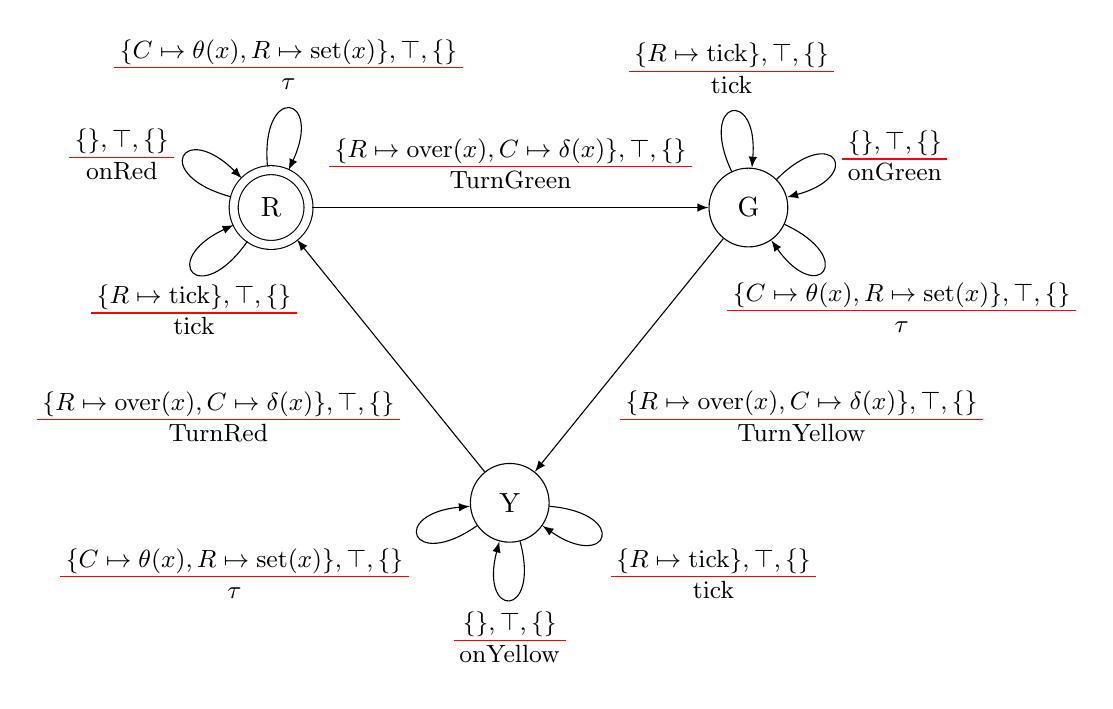
\begin{tikzpicture}

\node[state,initial] (v1) at (150:3.5) {R};
\node[state] (v2) at (30:3.5) {G};
\node[state] (v3) at (270:2) {Y};

\draw (v1) edge[dir=220] node[below] {\OTd{\act{tick}}{R \mapsto \act{tick}}{}} (v1);
\draw (v1) edge[dir=150] node[left] {\OTd{\act{onRed}}{}{}} (v1);
\draw (v1) edge[dir=80] node[above] {\OTd{\tau}{C \mapsto \theta\mpar{x}, R \mapsto \act{set}\mpar{x}}{}} (v1);
\draw (v1) edge node {\OTd{\act{TurnGreen}}{R \mapsto \act{over}\mpar{x}, C \mapsto \delta\mpar{x}}{}} (v2);
\draw (v2) edge[dir=100] node[above] {\OTd{\act{tick}}{R \mapsto \act{tick}}{}} (v2);
\draw (v2) edge[dir=30] node[right] {\OTd{\act{onGreen}}{}{}} (v2);
\draw (v2) edge[dir=320] node[xshift=1cm,below] {\OTd{\tau}{C \mapsto \theta\mpar{x}, R \mapsto \act{set}\mpar{x}}{}} (v2);
\draw (v2) edge node[pos=0.6] {\OTd{\act{TurnYellow}}{R \mapsto \act{over}\mpar{x}, C \mapsto \delta\mpar{x}}{}} (v3);
\draw (v3) edge[dir=340] node {\OTd{\act{tick}}{R \mapsto \act{tick}}{}} (v3);
\draw (v3) edge[dir=270] node {\OTd{\act{onYellow}}{}{}} (v3);
\draw (v3) edge[dir=200] node {\OTd{\tau}{C \mapsto \theta\mpar{x}, R \mapsto \act{set}\mpar{x}}{}} (v3);
\draw (v3) edge node[pos=0.4] {\OTd{\act{TurnRed}}{R \mapsto \act{over}\mpar{x}, C \mapsto \delta\mpar{x}}{}} (v1);

\end{tikzpicture}
}
\caption{The specification of a Traffic Light system}
\label{fig:tls}
\end{figure}


\begin{figure}[!tb]
%\centering
\scalebox{.75}{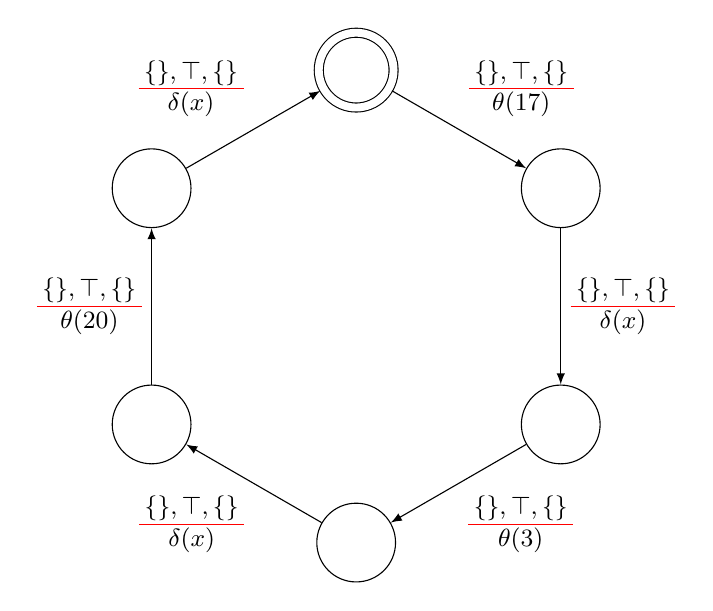
\begin{tikzpicture}

\node[state,initial] (v1) at (90:3) {};
\node[state] (v2) at (30:3) {};
\node[state] (v3) at (330:3) {};
\node[state] (v4) at (270:3) {};
\node[state] (v5) at (210:3) {};
\node[state] (v6) at (150:3) {};

\draw (v1) edge node {\OTd{\theta\mpar{17}}{}{}} (v2);
\draw (v2) edge node {\OTd{\delta\mpar{x}}{}{}} (v3);
\draw (v3) edge node {\OTd{\theta\mpar{3}}{}{}} (v4);
\draw (v4) edge node {\OTd{\delta\mpar{x}}{}{}} (v5);
\draw (v5) edge node {\OTd{\theta\mpar{20}}{}{}} (v6);
\draw (v6) edge node {\OTd{\delta\mpar{x}}{}{}} (v1);

\end{tikzpicture}
}
\scalebox{.75}{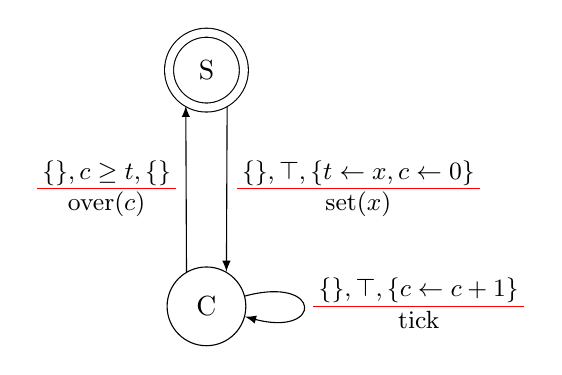
\begin{tikzpicture}

\node[state,initial] (v1) at (0,1.5) {S};
\node[state] (v2) at (0,-1.5) {C};

\draw (v1) edge[bend left,looseness=0] node {\OTd{\act{set}\mpar{x}}{}{t \gets x, c \gets 0}} (v2);
\draw (v2) edge[dir=0] node {\OTd{\act{tick}}{}{c \gets c + 1}} (v2);
\draw (v2) edge[bend left,looseness=0] node {\OTd{\act{over}\mpar{c}}{}[c \geq t]{}} (v1);

\end{tikzpicture}
}
\caption{(a) An example of controller component ~~  (b) An example of counter component}
\label{fig:ctlandcnt}
\end{figure}

\begin{figure}[!tb]
\centering
\scalebox{.75}{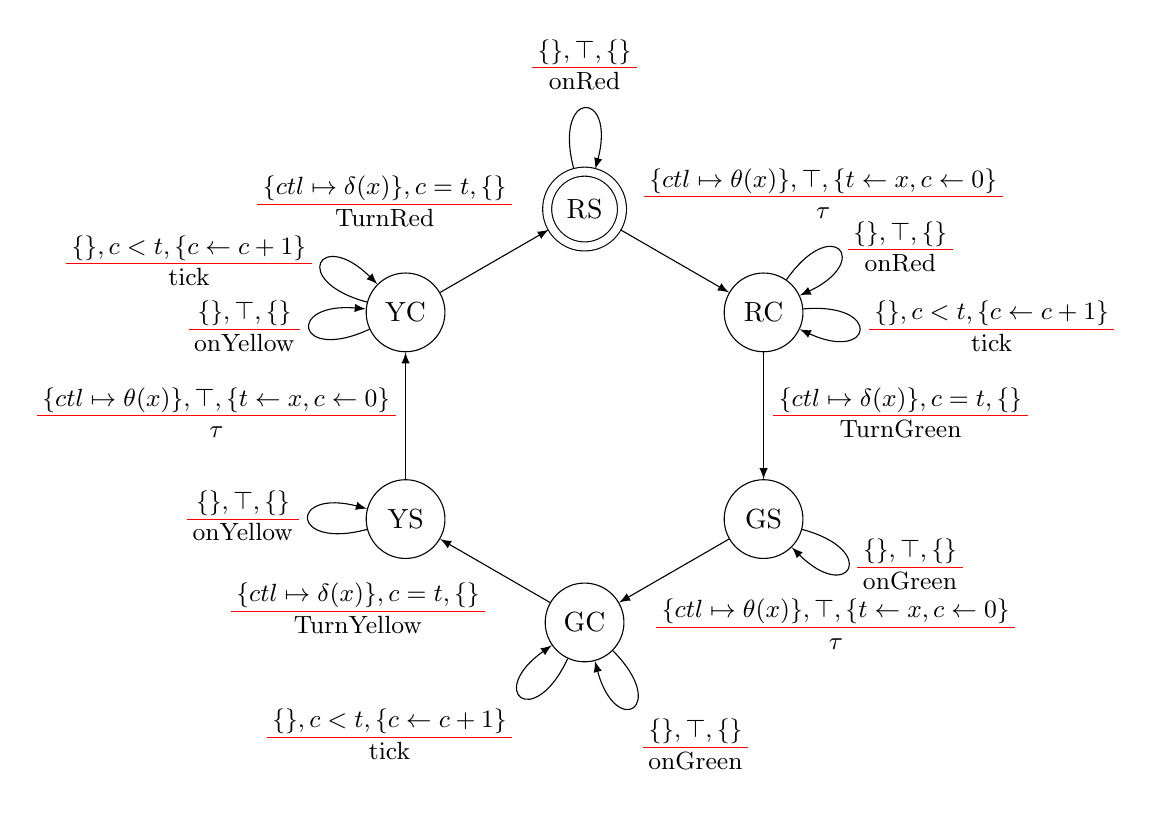
\begin{tikzpicture}[scale=0.75]

\node[state,initial] (v1) at (90:3.5) {RS};
\node[state] (v2) at (30:3.5) {RC};
\node[state] (v3) at (330:3.5) {GS};
\node[state] (v4) at (270:3.5) {GC};
\node[state] (v5) at (210:3.5) {YS}; 
\node[state] (v6) at (150:3.5) {YC};

\draw (v1) edge[dir=90] node {\OTd{\act{onRed}}{}{}} (v1);
\draw (v1) edge node[very near start] {\OTd{\tau}{ctl \mapsto \theta\mpar{x}}{t \gets x, c \gets 0}} (v2);
\draw (v2) edge[dir=40] node[right] {\OTd{\act{onRed}}{}{}} (v2);
\draw (v2) edge[dir=350] node[right] {\OTd{\act{tick}}{}[c < t]{c \gets c + 1}} (v2);
\draw (v2) edge node {\OTd{\act{TurnGreen}}{ctl \mapsto \delta\mpar{x}}[c = t]{}} (v3);
\draw (v3) edge[dir=330] node[right] {\OTd{\act{onGreen}}{}{}} (v3);
\draw (v3) edge node[near end] {\OTd{\tau}{ctl \mapsto \theta\mpar{x}}{t \gets x, c \gets 0}} (v4);
\draw (v4) edge[dir=300] node {\OTd{\act{onGreen}}{}{}} (v4);
\draw (v4) edge[dir=230] node {\OTd{\act{tick}}{}[c < t]{c \gets c + 1}} (v4);
\draw (v4) edge node {\OTd{\act{TurnYellow}}{ctl \mapsto \delta\mpar{x}}[c = t]{}} (v5);
\draw (v5) edge[dir=180] node {\OTd{\act{onYellow}}{}{}} (v5);
\draw (v5) edge node {\OTd{\tau}{ctl \mapsto \theta\mpar{x}}{t \gets x, c \gets 0}} (v6);
\draw (v6) edge[dir=190] node[left] {\OTd{\act{onYellow}}{}{}} (v6);
\draw (v6) edge[dir=150] node[left] {\OTd{\act{tick}}{}[c < t]{c \gets c + 1}} (v6);
\draw (v6) edge node[near end] {\OTd{\act{TurnRed}}{ctl \mapsto \delta\mpar{x}}[c = t]{}} (v1);

\end{tikzpicture}
}
\caption{The incomplete Specification Traffic Lights system}
\label{fig:tlf}
\end{figure}



\begin{figure}[!tb]
\centering
\scalebox{.75}{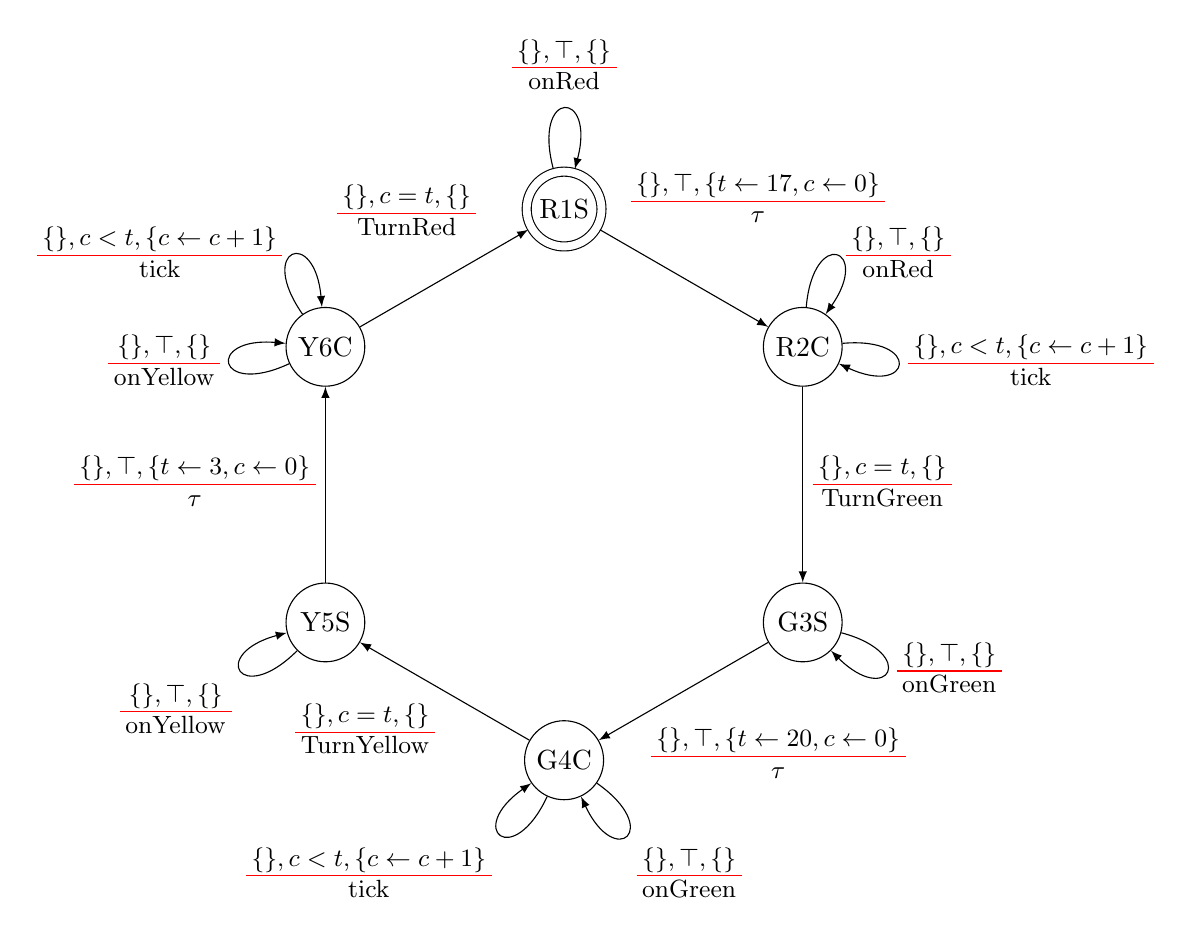
\begin{tikzpicture}

\node[state,initial] (v1) at (90:3.5) {R1S};
\node[state] (v2) at (30:3.5) {R2C};
\node[state] (v3) at (330:3.5) {G3S};
\node[state] (v4) at (270:3.5) {G4C};
\node[state] (v5) at (210:3.5) {Y5S};
\node[state] (v6) at (150:3.5) {Y6C};

\draw (v1) edge[dir=90] node {\OTd{\act{onRed}}{}{}} (v1);
\draw (v1) edge node[very near start] {\OTd{\tau}{}{t \gets 17, c \gets 0}} (v2);
\draw (v2) edge[dir=70] node[right] {\OTd{\act{onRed}}{}{}} (v2);
\draw (v2) edge[dir=350] node[right] {\OTd{\act{tick}}{}[c < t]{c \gets c + 1}} (v2);
\draw (v2) edge node {\OTd{\act{TurnGreen}}{}[c = t]{}} (v3);
\draw (v3) edge[dir=330] node[right] {\OTd{\act{onGreen}}{}{}} (v3);
\draw (v3) edge node[near end] {\OTd{\tau}{}{t \gets 20, c \gets 0}} (v4);
\draw (v4) edge[dir=310] node {\OTd{\act{onGreen}}{}{}} (v4);
\draw (v4) edge[dir=230] node {\OTd{\act{tick}}{}[c < t]{c \gets c + 1}} (v4);
\draw (v4) edge node {\OTd{\act{TurnYellow}}{}[c = t]{}} (v5);
\draw (v5) edge[dir=210] node {\OTd{\act{onYellow}}{}{}} (v5);
\draw (v5) edge node {\OTd{\tau}{}{t \gets 3, c \gets 0}} (v6);
\draw (v6) edge[dir=190] node[left] {\OTd{\act{onYellow}}{}{}} (v6);
\draw (v6) edge[dir=110] node[left] {\OTd{\act{tick}}{}[c < t]{c \gets c + 1}} (v6);
\draw (v6) edge node[near end] {\OTd{\act{TurnRed}}{}[c = t]{}} (v1);

\end{tikzpicture}
}
\caption{The full Traffic Lights system}
\label{fig:tlf}
\end{figure}


\section{A First Refinement Relation}\label{sec:refinement}

Similarly to FH-bisimulation~\cite{fhbisim} we are interested  in finding relations between states of to open automata that contain variables and holes. However here we want to build a refinement relation that  also guarantees that no deadlock is introduced when refining the automaton.
The refinement relation should be conditioned by the internal states of the automata. More precisely, a refinement relation characterizes when two states are related, this  characterisation is expressed as a predicate on the variables of the two automata.
Thus, a refinement relation has the following signature: \( S_1 \times S_2 \to \rformulas[V_1 \uplus V_2]\).

\TODO{check deadlock reduction/reducing in the literature}
We first define when a relation is deadlock reducing, before characterising a first simple refinement relation  to compare automata with identical holes.

\subsection{Deadlock Reduction, Reachability, and Composition}

A notion that is often used in the context of refinement is the notion of deadlock reduction. This property considers that two states related by a given relation and states that if one state can do a transition, then the other can do a transition too. This notion is not much interesting in the general case as there is a priori no relation between the two transitions. However, when the relation that relates states is a simulation, this will relate the possible transitions and the deadlock reduction will become a valuable property.

Next definition states that if $T_2$ is not in a deadlock position then $T_1$ can do a transition but not necessarily with the same input values. This is very weak but sufficient when composed with the def  of simulation.

\begin{definition}[Deadlock reduction]\label{def:dpwd}\\
Let \(\OAg[1]\) and \(\OAg[2]\) be two OAs.
A relation on OA configurations \(R: S_1 \times S_2 \to \rformulas[V_1 \uplus V_2]\) is deadlock reducing if  it satisfies the following\footnote{Note that variables of $T_1$ are existentially quantified in the proposition.}:
\begin{multline*}
 \forall \mpar{s_1, s_2} \in S_1 \times S_2,\\ V_1 \uplus V_2 \uplus \biguplus_\subbox{t_2 \in \fOT{s_2}} \fvars{t_2} \vdash \left(R\mpar{s_1, s_2} \wedge \bigvee_\subbox{t_2 \in \fOT{s_2}} \fguard{t_2} \implies \bigvee_\subbox{t_1 \in \fOT{s_1}} \fguard{t_1} \right)
\end{multline*}
\end{definition}

Because of the symbolic nature of OAs and their structure, in this definition,  the fact that a guard is true is sufficient to reason on the possible paths. This slightly simplifies the definition and makes the characterisation of transition that can be triggered very symbolic. An equivalent but more classical definition of deadlock reduction could be expressed as well. It states that if there is a transition that can be triggered in the first automaton, then there is a transition from the related state in the second automaton that can be triggered. This second definition is more verbose, in particular because of the multiple quantifiers over transitions and automaton state. The alternative definition is equivalent to this one when reasoning on a refinement relation (but not in general).

Unfortunately, this property is not compositional: the composition operator can itself introduce a deadlock. In other words, when filling the hole of two related automata with a third one, even if there is a deadlock reduction between the two original automata , there might not be a deadlock reduction in the composed ones. The same problem may arise when two related automata are composed in the same hole of a third one. 

This creates a conflict between deadlock reduction and the properties involving composition. One possible solution to avoid this conflict is to only consider a composition that do not introduce deadlocks, we will define such a composition below.
But before defining non-blocking composition, we first introduce a notion of state reachability for open automata. 
\begin{definition}[Reachability] \label{Def:Reach}
For any open automata \(A = \OAg\), a reachability predicate \(\reach{A}: S \to \rformulas[V]\) is any predicate on states that is valid on initial state, and preserved across transitions:
\[\sigma_0 \vdash \reach{A}\mpar{s_0}\quad\land\quad\forall t = \OTg \in T, \fvars{t} \vdash \left(\reach{A}\mpar{s} \wedge g \implies \reach{A}\mpar{s'}\psubst{\psi}\right)\]
\end{definition}
Reachability takes into account all paths, and can over-approximate the reachable configurations. 
From an automation point of view, finding the most precise reachability predicate for a given automata is not decidable because of the symbolic nature of open automata, but only an over-approximation is necessary. An automatic tool would only need to find an over approximation of reachability to reason on composition that is compatible with deadlock reduction. We call \emph{non-blocking composition} a composition that can be safely be used to compose open automata that are involved in a deadlock reducing relation.

\begin{definition}[Non-blocking composition]\label{Def:Non-blockcomp}
Let \(A_i = \OAg[i]\) with \( 0 \leq i \leq n\) be a family of open automata.
Let \(A = A_0\mdbrk{j_i \mapsto A_i \middle| 1 \leq i \leq n}\) and $A= \OAg$.

The composition \(A_0\mdbrk{j_i \mapsto A_i \middle| 1 \leq i \leq n}\) is non-blocking if   \(A \) has a reachability predicate such that, for each reachable configuration, if there is a possible transition in \(A_0\) then there is a possible transition in \(A\):
\[ \forall s = \mpar{s_0, s_1,..,s_n} \in S, V \uplus \biguplus_\subbox{t_0 \in \fOT{s_0}} \fvars{t_0} \vdash \left(\reach{A}\mpar{s} \wedge \bigvee_\subbox{t_0 \in \fOT{s_0}} \fguard{t_0} \implies \bigvee_\subbox{t \in \fOT{s}} \fguard{t} \right)\]
\end{definition}
Again we use guards to ensure that the transition can occur. It is not sufficient to ensure the existence of equivalent transitions in general, but it will be sufficient in the context of refinement.



\subsection{Refinement Relations for automata with the same holes}

We define here simulation between labelled transition systems to Hole-equal simulation  between  open automata that have exactly the same holes.
\begin{definition}[Hole-equal simulation]
Consider two OAs \(\OAg[1]\) and \(\OAg[2]\) with  \(J_1 = J_2\), the relation on configurations \(R: S_1 \times S_2 \to \rformulas[V_1 \uplus V_2]\) is a hole-\(\symb{equal}\) simulation from $S_1$ to $S_2$ if the following conditions hold: 
\item[(1)] \(\sigma_{01} \uplus \sigma_{02} \vdash R\mpar{s_{01}, s_{02}}\)
\item[(2)] \(\forall \mpar{s_1, s_2} \in S_1 \times S_2,\)\vspace{-8pt}
\noindent\begin{multline*}
\everymath{\displaystyle}\begin{array}{l}
		\bigsymb{\forall} t_1 = \OTx{1}{}{1}{1} \in \fOT{s_1}, \bigsymb{\exists} \mpar{t_{2x} = \OTx{2}{x}{2x}{2x} \in \fOT{s_2}}^{x \in X}, \\[10pt]
		\quad \mpar{\forall x \in X, J'_{2x}= J'_1} \\[2pt]
		\nwedge V_1 \uplus V_2 \uplus \fvars{t_1} \vdash\\
\hspace{5em} \left( R\mpar{s_1, s_2} \wedge g_1 \implies \operatorname*{\bigsymb{\bigvee}}_{x \in X} \mpar{\begin{array}{l}
			\alpha_1 = \alpha_{2x} \wedge \bigwedge_\subbox{j \in J'_{2x}} \beta_{1j} = \beta_{2xj} \\[12pt]
			\nwedge g_{2x} \wedge R\mpar{s'_1, s'_{2x}}\psubst{\psi_1 \uplus \psi_{2x}}
		\end{array}}\right)
	\end{array} 
%\\
%	\wedge \mpar{V_1 \uplus V_2 \uplus \biguplus_\subbox{t_2 \in \fOT{s_2}} \fvars{t_2} \vdash R\mpar{s_1, s_2} \wedge \bigvee_\subbox{t_2 \in \fOT{s_2}} \fguard{t_2} \implies \bigvee_\subbox{t_1 \in \fOT{s_1}} \fguard{t_1}}
\end{multline*}
\item[(3)] $R$ is deadlock reducing.
\end{definition}


Note in this definition, instead of matching an instantiated transition of the first automata to another instantiated transition of the second, it matches an open transition $t_1$ to a family of covering open transitions $t_{2x}^{x\in X}$. %Note also the second part of the conjunction of condition (2) expresses the deadlock reduction between automata (as introduced in Definition \ref{def:dpwd}).   

Intuitively, this means that for every pair of related
states $(s_1,s_2)$  of the two automata, and for every  transition of the first automaton from $s_1$, there is a set of matching transitions  of the second automaton  from $s_2$ such that the produced action match, the actions of the same holes and the successors are related after variable update. Our definition captures a simple kind of sub-classing of open automata with the same holes. It is stronger than a strict simulation since it matches a transition with a family of transitions. 
With such a relation we are able to check the refinement between two open automata with the same level of abstraction but specified differently, for example, by duplicating states, removing transitions,  reinforcing  guards, modifying variables. 
However, this refinement is inappropriate in the setting of composition which is the main advantage of the open automaton-based approach. 
\TODO{introduce somewhere refinement through composition} 
Refinement through composition  leads to a model in which composition can be used both to add new holes to a system and to fill holes, obtaining a system with less holes.
Next section will identify a refinement relation with the possibility to have different holes in the compared automata.



%Technically,  it expresses how the concepts from the abstract and the refined systems are linked together.

\TODO{add an example}

\TODO{refer to properties of section 6} We will show in Section~\ref{sec:prop} that this refinement relation has god properties in terms of transitivity, compositionality, reflexivity, etc.

\TODO{4 pages}

\section{A Refinement Relation that Takes Holes into Account}\label{sec:holes}
\TODO{3.5 pages}

Above we designed a refinement relation that compares OAs with the same holes, it ensures simulation at the automaton level, with symbolic evaluation of the guards and transitions. We want now to extend this to automata where the set of holes is not the same. A trivial use-case for this is filling a hole with a completely defined automaton. In this case, we want to ensure that the automaton with a filled hole is a refinement of the other automata: actions of the identical holes will be taken into account the same way, and filling the hole partially reduces the behaviour of the automaton.

The major challenge in this case is to maintain a form of transitivity while being able to take into account the actions of some of the holes. A naive definition of refinement would ensure that the holes that are identical in the two OAs are taken into account in the simulation. Unfortunately this does not work well with transitivity as if $A_1$ simulates $A_2$ and $A_2$ simulates $A_3$, and one hole appears in $A_3$ and in $A_1$ but not in $A_2$ then we have no proven property on the way $A_1$ and $A_3$ takes his hole into account, and in general  $A_1$ does not simulate $A_3$. The way we solve this issue is to remember in the simulation relation which holes have been compared. This way the relation is parameterized by the set of holes that belong to the two automata and are taken into account.
In practice, when performing successive refinements, we  keep track of which holes are in common at each step of refinement.

\TODO{say explicitly what is the difference in the formalisation compared to previous def}
\begin{definition}[Open automata refinement]\label{Def:OA-Refinement}
For two open automata\\ \(A_1 \defobject \OA{S_1}{s_{01}}{J_1}{V_1}{\sigma_{01}}{T_1}\) and \(A_2 \defobject \OA{S_2}{s_{02}}{J_2}{V_2}{\sigma_{02}}{T_2}\), \(A_1\) is a refinement of \(A_2\) tracking holes \(H\), noted \(\wrel{A_1}{A_2}{H}\), with \(H \subseteq J_1 \cap J_2\), if there is a relation $R: \mpar{S_1 \times S_2} \to \rformulas[V_1 \uplus V_2]$ such that:
\item[(1)] \(\sigma_{01} \uplus \sigma_{02} \vdash R\mpar{s_{01}, s_{02}}\)
\item[(2)] \(\forall \mpar{s_1, s_2} \in S_1 \times S_2,\)
\begin{multline*}
	\everymath{\displaystyle}\begin{array}{l}
		\bigsymb{\forall} \OTx{1}{}{1}{1} \in \fOT{s_1}, \bigsymb{\exists} \mpar{\OTx{2}{x}{2x}{2x} \in \fOT{s_2}}^{x \in X}, \\[12pt]
		\quad \mpar{\forall x \in X, J'_{2x} \cap H = J'_1 \cap H} \\[1pt]
		\nwedge V_1 \uplus V_2 \uplus \fvars{t_1} \vdash\\\hspace{5em} \mpar{R\mpar{s_1, s_2} \wedge g_1 \implies \operatorname*{\bigsymb{\bigvee}}_{x \in X} \mpar{\begin{array}{l}
			\alpha_1 = \alpha_{2x} \wedge \bigwedge_\subbox{j \in J'_{2x} \cap H} \beta_{1j} = \beta_{2xj} \\
			\nwedge g_{2x} \wedge R\mpar{s'_1, s'_{2x}}\psubst{\psi_1 \uplus \psi_{2x}}
		\end{array}}} 
	\end{array} 
\end{multline*}
\item[(3)] $R$ is deadlock reducing.

Giving \(R\) and \(H\) is sufficient to characterise the refinement, so we call \(\mpar{R, H}\) a hole-tracking simulation of \(A_1\) by \(A_2\).
Hole in \(H\) are called tracked holes.
\end{definition}
It is important to note that every action of the holes outside \(H\) is unconstrained in the related automata.
It is easy to see that the hole-equal simulation is a particular case of open automata refinement, when  $J_1=J_2=H$.


\TODO{example}

\section{Properties}\label{sec:prop}
\TODO{1.5 pages}


The first crucial property of  refinement  is that it is reflexive  and  transitive,  so  it  is  a  preorder on the set of open automata. This property enables stepwise refinement.


The relation  \(\wrel{}{}{H}\) is reflexive,  \(\wrel{A}{A}{H}\),  by taking $R\mpar{s_1, s_2} \mapsto \displaystyle\bigwedge_\subbox{v \in vars(s_1)} {v=v}$ to be $s_1= s_2$  and checking the above conditions (Definition \ref{Def:OA-Refinement}), we can see that the relation is indeed reflexive.


\begin{theorem}[Transitivity]
If $\wrel{A_1}{A_2}{H}$ and $\wrel{A_2}{A_3}{H'}$, then $\wrel{A_1}{A_3}{H\cap H'}$.
\end{theorem}

Appendix~\ref{sec:proof-transitivity} presents the proof. It is done classically by identifying the relation between $A_1$ and $A_3$ that is a refinement. What is less classical is the definition of this relation because it is a boolean formula. For each couple of states  $s_1$ and $s_3$ of $A_1$ and $A_3$ we build a a formula that defines the refinement relation. To do this, we take the disjunction of formulas relating $s_1$ and $s_3$, and passing by all states $s_2$ of $A_2$. More precisely, we define a relation of the following form:
  \[R_{13}(s_1,s_3)=\bigvee_{s_2\in S_2}\mpar{R_{12}(s_1,s_2) \land R_{23}(s_2,s_3) } \]
We then prove that this relation defines is a refinement, according to Definition~\ref{Def:OA-Refinement}.




\TODO{find an informal introduction to the following:}
The composition of $A_1$ and $A_3$ is a refinement of the composition of $A_2$ and $A_3$ provided $A_1$ is a refinement of $A_2$ and the hole in which we are composing inside $A_1$ and $A_2$ is tracked by the refinement relation.

\begin{theorem}[Context refinement]
Let $A_1$, $A_2$ and $A_3$ be three open automata with $\wrel{A_1}{A_2}{H}$. 
Let $J_3$ be the set of holes of $A_3$.
Suppose that \(k \in H\) and that \(A_1\subst{A_3}{k}\) is non-blocking.
We have: \[\wrel{A_1\subst{A_3}{k}}{A_2\subst{A_3}{k}}{J_3 \uplus H \setminus \mbrc{k}}\]
\end{theorem}

\begin{theorem}[Congruence]
Let $A_1$, $A_2$ and $A_3$ be three open automata with $\wrel{A_2}{A_3}{H}$. 
Suppose that \(k \in H\) and that \(A_1\subst{A_2}{k}\) is non-blocking.
We have: \[\wrel{A_1\subst{A_2}{k}}{A_1\subst{A_3}{k}}{J_1 \uplus H \setminus \mbrc{k}}\]
\end{theorem}
- composition is a refinement (under which condition? non-blocking composition?)

- what is the property wrt deadlocks?

- congruence? a[b/j] if $a'$ refines $a$ and if $b'$ refines $b$?

- relation with fh bisimulation



\section{Conclusion}\label{sec:ccl}
\TODO{0.5 pages}


\section{a recuperer si on se rend compte que c'est utile}
When we will introduce refinements in Section \ref{sec:prelref}, setting an undefined variable will be considered a valid refinement, for instance a \(5\) bits register is a particular \(n\) bits register.


\appendix

\section{Proof of Transitivity}\label{sec:proof-transitivity}
\begin{quote}
If $\wrel{A_1}{A_2}{H}$ and $\wrel{A_2}{A_3}{H'}$, then $\wrel{A_1}{A_3}{H\cap H'}$.
\end{quote}
\proof 
If $\wrel{A_1}{A_2}{H}$ then there is $R_{12}$ a relation between states
of $A_1$ and of $A_2$;  If $\wrel{A_2}{A_3}{H'}$ then there is $R_{23}$ a relation between states of $A_2$ and of $A_3$. We build a relation between
 states of $A_1$ and of $A_3$ as follows:  for each pair of states $s_1$, $s_3$, for each state $s_2$ such that $R_{12}$ relates $s_1$ and $s_2$, and $R_{23}$ relates $s_2$ and $s_3$.
Let $R_{13}$ be the relation:\\
  \[R_{13}(s_1,s_3)=\bigvee_{s_2\in S_2}\mpar{R_{12}(s_1,s_2) \land R_{23}(s_2,s_3) } \]

We will show that $\wrel{A_1}{A_3}{H\cap H'}$ by exhibiting  $R_{13}$ as a hole-tracking simulation of $A_1$ by  $A_3$.

We have to prove that the relation $R_{13}$ satisfies the three conditions of the definition of a refinement of open automata.
\begin{enumerate}
\item Firstly, we have to $R_{13}$ satisfies initial configurations:
\[\sigma_{01} \uplus \sigma_{03} \vdash R_{13} \mpar{s_{01}, s_{03}}\]
By knowing that substitutions only have an effect on the variables of the open automaton they belong to, they also produce terms containing only variables of the open automaton they belong to. We have:
\begin{align*}
\mpar{\sigma_{01} \uplus \sigma_{02} \vdash R_{12}\mpar{s_{01}, s_{02}}} \wedge \mpar
{\sigma_{02} \uplus \sigma_{03} \vdash R_{23}\mpar{s_{02}, s_{03}}}&\implies\\
R_{12}\mpar{s_{01},s_{02}}\psubst{\sigma_{01} \uplus \sigma_{02}} \wedge R_{23}\mpar{s_{02}, s_{03}}\psubst{\sigma_{02} \uplus \sigma_{03}}&\implies\\
R_{12}\mpar{s_{01},s_{02}}\psubst{\sigma_{01} \uplus \sigma_{02} \uplus \sigma_{03}} \wedge R_{23}\mpar{s_{02}, s_{03}}\psubst{\sigma_{01} \uplus \sigma_{02} \uplus \sigma_{03}}&\implies\\ 
\underbrace{R_{12}\mpar{s_{01},s_{02}}\wedge R_{23}\mpar{s_{02}, s_{03}}}_{\implies R_{13} \mpar{s_{01}, s_{03}}}\psubst{\sigma_{01} \uplus \sigma_{02} \uplus \sigma_{03}} %&\implies\\
 \end{align*}
Since $\sigma_{02}$ has no effect on variables of $s_{01}$ and $s_{03}$ thus we get the expected result.

\item Secondly, we need to prove that for any open transition $t_1$ in $T_1$  originating from $s_1$:
\begin{align*}
\OTx{1}{}{1}{1} \in \fOT{s_1}
\end{align*}
there exists an indexed family of OTs originating from $s_{3}$: 
\begin{multline*}
V_1 \uplus  V_3 \uplus \fvars{t_1}
\vdash\\\hspace{2em}
\mpar{R_{13}\mpar{s_1, s_3} \wedge g_1 \implies 
\operatorname*{\bigsymb{\bigvee}}_{z \in Z}
\mpar{\everymath{\displaystyle}
\begin{array}{l}
\alpha_1=\alpha_{3z}\wedge \bigwedge_\subbox{j \in J'_{3z} \cap (H\cap H')} \beta_{1j}=\beta_{3jz} \wedge \\g_{3z}\wedge 
{R_{12}\mpar{s'_1,s'_{3z}}}\psubst{\psi_1  \uplus \psi_{3z}}
\end{array}}}
\end{multline*}	
\medskip
 Consider $\mpar{s_{1}, s_{3}} \in R_{13}$ then there is a set of states $(s_{2p})^{p\in P}$ of $A_2$ relating  $s_{1}$ and $s_{3}$:
\[R_{13}(s_1,s_3)=\bigvee_{{p\in P}
}\mpar{R_{12}\mpar{s_1,s_{2p}} \wedge R_{23}\mpar{s_{2p},s_3}} \]

Let's consider any $s_{2p} \in (s_{2p})^{p\in P}$. We have on one side,  for any open transition $t_1$ in $T_1$  originating from $s_1$:
\begin{align*}
\OTx{1}{}{1}{1} \in \fOT{s_1}
\end{align*}
there exists an indexed family of OTs originating from $s_{2p}$: 
\begin{align*}
\mpar{\OTx{2p}{x}{2px}{2px} \in \fOT{s_{2p}}}^{x \in X_p} 
\end{align*}
such that $\forall x \in X, J'_{2px} \cap H = J'_1 \cap H$ and
\begin{multline*}
%\everymath{\displaystyle}
V_1 \uplus V_2 \uplus \fvars{t_1} \vdash\\ \mpar{R_{12}\mpar{s_1, s_{2p}} \wedge g_1 \implies \operatorname*{\bigsymb{\bigvee}}_{x \in X_p} \mpar{\everymath{\displaystyle}
\begin{array}{l}
			\alpha_1 = \alpha_{2px} \wedge \bigwedge_\subbox{j \in J'_{2px} \cap H} \beta_{1j} = \beta_{2pxj} \nwedge\\
			 g_{2px} \wedge R_{12}\mpar{s'_1, s'_{2px}}\psubst{\psi_1 \uplus \psi_{2px}}
		\end{array}}} 
\end{multline*}		
Adding to both sides of the implication the predicate $R_{23}\mpar{s_{2p},s_3}$ we get: 
\begin{multline*}
V_1 \uplus V_2 \uplus V_3  \uplus \fvars{t_1} \vdash\\
R_{12}\mpar{s_1, s_{2p}} \wedge R_{23}\mpar{s_{2p},s_3} \wedge g_1 \implies\hspace{5.5cm}\\ \operatorname*{\bigsymb{\bigvee}}_{x \in X} \mpar{\everymath{\displaystyle}
\begin{array}{l}
			\alpha_1 = \alpha_{2px} \wedge \bigwedge_\subbox{j \in J'_{2px} \cap H} \beta_{1j} = \beta_{2pxj} \land\\
			 g_{2px} \wedge R_{12}\mpar{s'_1, s'_{2px}}\psubst{\psi_1 \uplus \psi_{2px}} \land R_{23}\mpar{s_{2p},s_3}
		\end{array}} \qquad (*) 
\end{multline*}	
On the other side, according the relation between $A_2$ and $A_3$ we have for any open transition $t_{2px}$ in $T_2$ originating from $s_{2p}$:
\begin{align*}
\OTx{2p}{x}{2px}{2px} \in \fOT{s_{2p}}
\end{align*}
there exists an indexed family of OTs originating from $s_3$: 
\begin{align*}
\mpar{\OTx{3}{pxy}{3pxy}{3pxy} \in \fOT{s_3}}^{y \in Y} 
\end{align*}
such that $\forall y \in Y, J'_{2px} \cap H' = J'_{3pxy} \cap H'$ and
\begin{multline*}
%\everymath{\displaystyle}
V_2 \uplus V_3 \uplus \fvars{t_{2px}} \vdash\\
R_{23}\mpar{s_{2p}, s_{3}} \wedge g_{2px} \implies \hspace{7cm}\\ \operatorname*{\bigsymb{\bigvee}}_{y \in Y} \mpar{\everymath{\displaystyle}
\begin{array}{l}
			 \alpha_{2px}=\alpha_{3pxy} \wedge \bigwedge_\subbox{j \in J'_{3pxy} \cap H'} \beta_{2pxj}=\beta_{3pxyj} \nwedge \\
			g_{3pxy} \wedge R_{23}\mpar{s'_{2px}, s'_{3xy}}\psubst{\psi_{2px} \uplus \psi_{3pxy}}
		\end{array}}  \qquad (**)
\end{multline*}

From the  two previous cases: 
$\forall x \in X, J'_{2px} \cap H = J'_1 \cap H$ and
$\forall y \in Y, J'_{2px} \cap H' = J'_{3pxy} \cap H'$ we conclude:
$\forall x \in X, \forall y \in Y,  J'_1 \cap (H \cap H') = J'_{3pxy} \cap (H\cap H')$ \\

In addition, by combining  formula $(**)$ and $(*)$, we get: 
\begin{multline*}
V_1 \uplus V_2 \uplus V_3  \uplus \fvars{t_1}\uplus \fvars{t_{2px}} \vdash\\
R_{12}\mpar{s_1, s_{2p}} \wedge R_{23}\mpar{s_{2p},s_3} \wedge g_1 \implies \hspace{4.5cm}\\\operatorname*{\bigsymb{\bigvee}}_{x \in X} \mpar{\everymath{\displaystyle}
\begin{array}{l}
			\alpha_1 = \alpha_{2px} \wedge \bigwedge_\subbox{j \in J'_{2px} \cap H} \beta_{1j} = \beta_{2pxj}  \wedge R_{12}\mpar{s'_1, s'_{2px}}\psubst{\psi_1 \uplus \psi_{2px}} \\ 
\land
		\operatorname*{\bigsymb{\bigvee}}_{y \in Y} \mpar{\everymath{\displaystyle}
\begin{array}{l}
			 \alpha_{2px}=\alpha_{3pxy} \wedge \bigwedge_\subbox{j \in J'_{3pxy} \cap H'} \beta_{2pxj}=\beta_{3pxyj} \nwedge\\
			 g_{3pxy} \wedge R_{23}\mpar{s'_{2px}, s'_{3pxy}}\psubst{\psi_{2px} \uplus \psi_{3pxy}}
		\end{array}}	
		\end{array}} 
\end{multline*}		
With  the rearrangement of the formula, we get:
\begin{multline*}
V_1 \uplus V_2 \uplus V_3  \uplus \fvars{t_1}\uplus \fvars{t_{2px}}  \vdash\\
R_{12}\mpar{s_1, s_{2p}} \wedge R_{23}\mpar{s_{2p},s_3} \wedge g_1 \implies 
\hspace{5.5cm}\\
\operatorname*{\bigsymb{\bigvee}}_{x \in X} 
\operatorname*{\bigsymb{\bigvee}}_{y \in Y}
\mpar{\everymath{\displaystyle}
\begin{array}{l}
\alpha_1=\alpha_{3pxy}\wedge \bigwedge_\subbox{j \in J'_{3pxy} \cap (H\cap H')} \beta_{1j}=\beta_{3jpxy} \wedge g_{3pxy}\wedge \\
R_{12}\mpar{s'_1, s'_{2px}}\psubst{\psi_1 \uplus \psi_{2px}} \wedge R_{23}\mpar{s'_{2px}, s'_{3pxy}}\psubst{\psi_{2px} \uplus \psi_{3pxy}}
\end{array}}
\end{multline*}	

Because of the domain of the substitutions of the relations, the formula can be re-written:
\begin{multline*}
V_1 \uplus V_2 \uplus V_3  \uplus \fvars{t_1}\uplus \fvars{t_{2px}} \vdash\\
R_{12}\mpar{s_1, s_{2p}} \wedge R_{23}\mpar{s_{2p},s_3} \wedge g_1 \implies 
\hspace{5.5cm}\\
\operatorname*{\bigsymb{\bigvee}}_{x \in X} 
\operatorname*{\bigsymb{\bigvee}}_{y \in Y}
\mpar{\everymath{\displaystyle}
\begin{array}{l}
\alpha_1=\alpha_{3pxy}\wedge \bigwedge_\subbox{j \in J'_{3pxy} \cap (H\cap H')} \beta_{1j}=\beta_{3jpxy} \wedge g_{3pxy}\wedge \\
\mpar{R_{12}\mpar{s'_1, s'_{2px}} \wedge R_{23}\mpar{s'_{2px}, s'_{3pxy}}}\psubst{\psi_1 \uplus \psi_{2px} \uplus \psi_{3pxy}}
\end{array}}
\end{multline*}
The formula is valid for all $s_{2p} \in (s_{2p})^{p\in P}$. To build $R_{13}$ we need to rely on the disjunction of all possible paths to relate $s_1$ and $s_3$, which leads to\\ ${\displaystyle R_{13}(s_1,s_3)=\bigvee_{{p\in P}}\mpar{R_{12}\mpar{s_1,s_{2p}} \wedge R_{23}\mpar{s_{2p},s_3}}}$.
\begin{multline*}
V_1 \uplus V_2 \uplus V_3  \uplus \fvars{t_1} \uplus  \biguplus_\subbox{p \in P} \fvars{t_{2px}} \vdash\\
\operatorname*{\bigsymb{\bigvee}}_{p\in P} \mpar{R_{12}\mpar{s_1, s_{2p}} \wedge R_{23}\mpar{s_{2p},s_3} \wedge g_1} \implies 
\hspace{5.5cm}\\
\operatorname*{\bigsymb{\bigvee}}_{p\in P}
\operatorname*{\bigsymb{\bigvee}}_{x \in X} 
\operatorname*{\bigsymb{\bigvee}}_{y \in Y}
\mpar{\everymath{\displaystyle}
\begin{array}{l}
\alpha_1=\alpha_{3pxy}\wedge \bigwedge_\subbox{j \in J'_{3pxy} \cap (H\cap H')} \beta_{1j}=\beta_{3jpxy} \wedge g_{3pxy}\wedge \\
\underbrace{R_{12}\mpar{s'_1, s'_{2px}} \wedge R_{23}\mpar{s'_{2px}, s'_{3pxy}}}_{\implies R_{13}\mpar{s'_1,s'_{3pxy}}}\psubst{\psi_1 \uplus \psi_{2px} \uplus \psi_{3pxy}}
\end{array}}
\end{multline*}
Indeed, since $\psi_{2px}$ has no effect on variables of $A_1$ and $A_3$ we have:
\begin{align*}
R_{12}\mpar{s'_1, s'_{2px}} \wedge R_{23}\mpar{s'_{2px}, s'_{3pxy}}\psubst{\psi_1 \uplus \psi_{2px} \uplus \psi_{3pxy}}  \\  
\implies R_{13}\mpar{s'_1,s'_{3pxy}}
\psubst{\psi_1 \uplus \psi_{2px} \uplus \psi_{3pxy}}  \\ 
\implies R_{13}\mpar{s'_1,s'_{3pxy}}\psubst{\psi_1  \uplus \psi_{3pxy}}
\end{align*}
This allows us to conclude that the family of open transitions of $A_3$ indexed over $p$, $x$,  and $y$ simulates the original open transition  with note that $\psi_{2px}$ has no effect on variables of $A_1$ and $A_3$:
\begin{multline*}
V_1  \uplus V_3  \uplus \fvars{t_1} \vdash\\
R_{13}(s_1,s_3)  \wedge g_1 \implies 
\hspace{5.5cm}\\
\operatorname*{\bigsymb{\bigvee}}_{p\in P}
\operatorname*{\bigsymb{\bigvee}}_{x \in X} 
\operatorname*{\bigsymb{\bigvee}}_{y \in Y}
\mpar{\everymath{\displaystyle}
\begin{array}{l}
\alpha_1=\alpha_{3pxy}\wedge \bigwedge_\subbox{j \in J'_{3pxy} \cap (H\cap H')} \beta_{1j}=\beta_{3jpxy} \\ \wedge g_{3pxy} 
{\wedge R_{13}\mpar{s'_1,s'_{3pxy}}}\psubst{\psi_1  \uplus \psi_{3pxy}}
\end{array}}
\end{multline*}
Overall, we have a family of open transitions $t^{p\in P,x\in X,y\in Y}_{pxy} \subseteq T_3$ that should simulate $t_1$. All  combinations of elements in $P$, $X$, and $Y$ provide a set $Z$ of  open transitions.  This allows us to get the desired conclusion, that there is a set of  open transitions indexed over $Z$:
%This provides the desired conclusion:\\
\begin{multline*}
V_1 \uplus  V_3 \uplus \fvars{t_1}
\vdash\\\hspace{2em}
\mpar{R_{13}\mpar{s_1, s_3} \wedge g_1 \implies 
\operatorname*{\bigsymb{\bigvee}}_{z \in Z}
\mpar{\everymath{\displaystyle}
\begin{array}{l}
\alpha_1=\alpha_{3z}\wedge \bigwedge_\subbox{j \in J'_{3z} \cap (H\cap H')} \beta_{1j}=\beta_{3jz} \wedge \\g_{3z}\wedge 
{R_{13}\mpar{s'_1,s'_{3z}}}\psubst{\psi_1  \uplus \psi_{3z}}
\end{array}}}
\end{multline*}	
\medskip
\item Finally, we need to prove the satisfaction of the  deadlock reducing condition. According to the refinement relation relating   $A_2$ and $A_3$ we have for all $\mpar{s_{2p}, s_3} \in S_2 \times S_3$:
\begin{multline*}
 V_2 \uplus V_3 \uplus \biguplus_\subbox{t_3 \in \fOT{s_3}} \fvars{t_3} \vdash \left(R_{23}\mpar{s_{2p}, s_3} \wedge \bigvee_\subbox{t_3 \in \fOT{s_3}} \fguard{t_3} \implies \bigvee_\subbox{t_{2p} \in \fOT{s_{2p}}} \fguard{t_{2p}} \right)
\end{multline*}
By adding the term $R_{12}\mpar{s_1,s_{2p}}$ to both sides of the implication, we get:
\begin{multline*}
V_1 \uplus V_2 \uplus V_3 \uplus \fvars{t_{2p}} \uplus \biguplus_\subbox{t_3 \in \fOT{s_3}} \fvars{t_3} \vdash \\
R_{12}\mpar{s_1,s_{2p}}\wedge R_{23}\mpar{s_{2p}, s_3} \wedge \bigvee_\subbox{t_3 \in \fOT{s_3}} \fguard{t_3} \implies R_{12}\mpar{s_1,s_{2p}}\wedge \bigvee_\subbox{t_{2p} \in \fOT{s_{2p}}} \fguard{t_{2p}} 
\end{multline*}
This is valid for all $s_{2p} \in (s_{2p})^{p\in P}$ then we have:
\begin{multline*}
V_1 \uplus V_2 \uplus V_3 \uplus \biguplus_\subbox{p \in P} \fvars{t_{2p}} \uplus \biguplus_\subbox{t_3 \in \fOT{s_3}} \fvars{t_3} \vdash \\
\operatorname*{\bigsymb{\bigvee}}_{p\in P}\mpar{
R_{12}\mpar{s_1,s_{2p}}\wedge R_{23}\mpar{s_{2p}, s_3} \wedge \bigvee_\subbox{t_3 \in \fOT{s_3}} \fguard{t_3} \implies R_{12}\mpar{s_1,s_{2p}}\wedge \bigvee_\subbox{t_{2p} \in \fOT{s_{2p}}} \fguard{t_{2p}}} 
\end{multline*}
This results in:
\begin{multline*}
V_1 \uplus V_2 \uplus V_3 \uplus\biguplus_\subbox{p \in P} \fvars{t_{2p}} \uplus \biguplus_\subbox{t_3 \in \fOT{s_3}} \fvars{t_3} \vdash \\
R_{13}\mpar{s_1,s_3} \wedge \bigvee_\subbox{t_3 \in \fOT{s_3}} \fguard{t_3} \implies \operatorname*{\bigsymb{\bigvee}}_{p\in P}\mpar{ R_{12}\mpar{s_1,s_{2p}}\wedge \bigvee_\subbox{t_{2p} \in \fOT{s_{2p}}} \fguard{t_{2p}}} 
\end{multline*}
Yet according to the relation between $A_1$ and $A_2$ we have  for all $\mpar{s_1, s_{2p}} \in S_1 \times S_2$:
\begin{multline*}
 V_1 \uplus V_2 \uplus \biguplus_\subbox{t_{2p} \in \fOT{s_{2p}}} \fvars{t_{2p}} \vdash R_{12}\mpar{s_1, s_{2p}} \wedge \bigvee_\subbox{t_{2p} \in \fOT{s_{2p}}} \fguard{t_{2p}} \implies \bigvee_\subbox{t_1 \in \fOT{s_1}} \fguard{t_1} 
\end{multline*}



This formula is valid for all $s_{2p} \in (s_{2p})^{p\in P}$,  thus we can state the following:
\begin{multline*}
 V_1 \uplus V_2 \uplus \biguplus_{\mathclap{\substack{t_{2p} \in \fOT{s_{2p}}\\ p \in P}}} \fvars{t_{2p}} 
\vdash \\
\operatorname*{\bigsymb{\bigvee}}_{p\in P}\mpar{R_{12}\mpar{s_1, s_{2p}} \wedge \bigvee_\subbox{t_{2p} \in \fOT{s_{2p}}} \fguard{t_{2p}} }  \implies \bigvee_\subbox{t_1 \in \fOT{s_1}} \fguard{t_1}
\end{multline*}
By using transitive property of implication on formula obtained form both relations and by removing the $A_2$ variables that have not effect on   $A_1$ et  $A_3$, we get the desired result:
\begin{multline*}
V_1 \uplus V_3 \uplus \biguplus_\subbox{t_3 \in \fOT{s_3}} \fvars{t_3}
\vdash R_{13}\mpar{s_1,s_3} \wedge \bigvee_\subbox{t_3 \in \fOT{s_3}} \fguard{t_3}
\implies \bigvee_\subbox{t_1 \in \fOT{s_1}} \fguard{t_1}
\end{multline*}

\end{enumerate}

~\qed















\section{Proof of Context Refinement}


\begin{quote}
Suppose that $\wrel{A_1}{A_2}{H}$, \(k \in H\) and that \(A_1\subst{A_3}{k}\) is non-blocking.
We have: \[\wrel{A_1\subst{A_3}{k}}{A_2\subst{A_3}{k}}{J_3 \uplus H \setminus \mbrc{k}}\]
\end{quote}

\TODO{The subtlety here is that the original relation implies that valuations in A3 are equal (ie the value for each variable are the same in both valuations, modulo renaming), after a transition we should obtain ``equal'' valuations because Post are deterministic}

\proof
Let us denote by $A_{13}$ (resp. $A_{23}$) the open automaton resulting from $A_1\subst{A_3}{k}$ (resp. $A_2\subst{A_3}{k}$),  to prove the theorem it is sufficient to prove that there exists a relation between states of the two open automata that satisfies the conditions of the Definition \ref{Def:OA-Refinement}. 

We denote $A_1=  \OA{S_1}{s_{01}}{J_1}{V_1}{\sigma_{01}}{T_1}$ and \(A_2 \defobject \OA{S_2}{s_{02}}{J_2}{V_2}{\sigma_{02}}{T_2}\) and $A_3 = \OA{S_3}{s_{03}}{J_3}{V_3}{\sigma_{03}}{T_3}$. The proof requires  to rename the variables of one instance of the two $A_3$ automata to avoid clashes in variable names (this is required by the definition of refinement). In practice we will use superscripts ${}^1$ and ${}^2$ to distinguish elements of the two instances of $A_3$.

Let $R$ be the refinement relation relating states of $A_1$ and $A_2$. 
Let us denote with $t^1$ and $t^2$  the elements of $A_1$ and $A_2$ respectively.
Consider any two states $s_{13} = \mpar{s_1,s^1_3}$ and $s_{23} = \mpar{s_2,s^2_3}$ ($s^1_3$ and $s^2_3$  are the same with renaming). We define a relation $R'$ relating states of $s_{13}$ and $s_{23}$ as follows:
\[ R' \mpar{s_{13}, s_{23}} = R\mpar{s_{1}, s_{2}} \wedge \reach{A_{13}}\mpar{s_{13}} \wedge \bigwedge_\subbox{v_3\in V_3}
 v^1_3=v^2_3\wedge s^1_3 = s^2_3\]


We want to prove that $\mpar{R', H\uplus J_3 \setminus\{k\}}$ is a hole-tracking simulation of $A_{13}$ and $A_{23}$. In the following we denote $H'=H\cup J_3 \setminus\{k\}$.
\begin{enumerate}
\item First, we have to prove the relation for initial states:
\[\sigma_{013} \uplus \sigma_{023} \vdash R'\mpar{s_{013}, s_{023}}\]
with $\sigma_{013} = \sigma_{01} \uplus \sigma_{03}^1$, $\sigma_{023} = \sigma_{02} \uplus \sigma_{03}^2$, $s_{013}=(s_{01},s_{03}^1)$, and $s_{023}=(s_{02},s_{02}^2)$.\\
By using the fact that $R$ relates initial configurations of  $A_1$ and $A_2$, we have  the following statement:
$\mpar{\sigma_{01} \uplus \sigma_{02} \vdash R\mpar{s_{01}, s_{02}}}$,  and based on the  fact that initial states are reachable $\sigma_{013} \vdash \reach{A_{13}}\mpar{s_{013}}$ we have 
\[ \mpar{\sigma_{01} \uplus \sigma_{02} \vdash R\mpar{s_{01}, s_{02}}} \wedge 
\mpar{\sigma_{013} \vdash \reach{A_{13}}\mpar{s_{013}}}\]

Considering that initial valuations $\sigma_{03}^1$ and $\sigma_{03}^2$ associate the same values to the ``same'' variables modulo renaming, so the following holds:\\ $\left(\,\,{\displaystyle \bigwedge_\subbox{v_3\in V_3} v^1_3=v^2_3\wedge s^1_3 = s^2_3}\right)\psubst{\sigma_{03}^1 \uplus \sigma_{03}^2 }$.

Additionally, because  the domains of the substitution function are disjoint, the substitution function has an effect only on the related elements,  we get:
\begin{align*}
& \mpar{\sigma_{01} \uplus \sigma_{02} \vdash R\mpar{s_{01}, s_{02}}} \wedge 
\mpar{\sigma_{013} \vdash \reach{A_{13}}\mpar{s_{013}}}\\
\implies & R\mpar{s_{01}, s_{02}}\psubst{ \sigma_{01} \uplus \sigma_{02}} \wedge \reach{A_{13}}\mpar{s_{013}} \psubst{\sigma_{013}} \land \mpar{\,\,\bigwedge_\subbox{v_3\in V_3} v^1_3=v^2_3\wedge s^1_3 = s^2_3}\psubst{\sigma_{03}^1 \uplus \sigma_{03}^2 }\\
\implies & \mpar{R\mpar{s_{01}, s_{02}} \wedge \reach{A_{13}}\mpar{s_{013}}  \wedge \bigwedge_\subbox{v_3\in V_3}  v^1_3=v^2_3\wedge s^1_3 = s^2_3} \psubst{ \sigma_{01} \uplus \sigma_{02} \uplus \sigma^1_{03}\uplus \sigma^2_{03}\uplus \sigma_{013} }\\
\implies & \sigma_{013} \uplus \sigma_{023} \vdash R'\mpar{s_{013}, s_{023}}
\end{align*}
\item Second, we need to prove for any OT $t_{13}$ in $T_{13}$ originating from $s_{13}$:
\begin{align*}
		&  \OTx{13}{}{13}{13} \in \fOT{s_{13}}
\end{align*}		
there exists an indexed family $t_{23x}$ of OTs originating from $s_{23}$ that simulate it: 
\begin{align*}
		&  \mpar{\OTx{23}{x}{23x}{23x} \in \fOT{s_{23}}}^{x \in X}
\end{align*}	
\begin{align*}		
		& \text{such that } \mpar{\forall x \in X, J'_{23x} \cap H' = J'_{13} \cap H'} \text{ and }\\
		&  V_{13} \uplus V_{23} \uplus \fvars{t_{13}} \vdash R'\mpar{s_{13}, s_{23}} \wedge g_{13} \implies \operatorname*{\bigsymb{\bigvee}}_{x \in X} \mpar{\everymath{\displaystyle}\begin{array}{l}
			\alpha_{13} = \alpha_{23x} \wedge \bigwedge_\subbox{j \in J'_{23x} \cap H'} \beta_{13j} = \beta_{23xj} \wedge\\[12pt]
			 g_{23x} \wedge R'\mpar{s'_{13}, s'_{23x}}\psubst{\psi_{13} \uplus \psi_{23x}}
		\end{array}} 
	\end{align*}
Recall that by definition of composition and open automata refinement we have: 
\begin{align*}
&V_{13}= V_1\uplus V^1_3 \text{ and }
V_{23}= V_2\uplus V^2_3\\
& H' \subseteq J_3\uplus \mpar{J_1 \cap J_2} \setminus \{k\} = \mpar{J_3\uplus J_1 \setminus \{k\} } \cap \mpar{J_3\uplus J_2 \setminus \{k\}} \\
\end{align*}
First of all, we have by hypothesis $\wrel{A_1}{A_2}{H}$, then for any open transition $t_1$ in $T_1$  originating from $s_1$:
\begin{align*}
\OTx{1}{}{1}{1} \in \fOT{s_1}
\end{align*}
there exists an indexed family of OTs originating from $s_{2}$: 
\begin{align*}
\mpar{\OTx{2}{x}{2x}{2x} \in \fOT{s_{2}}}^{x \in X} 
\end{align*}
such that $\forall x \in X, J'_{2x} \cap H = J'_1 \cap H$ and
\begin{multline*}
%\everymath{\displaystyle}
V_1 \uplus V_2 \uplus \fvars{t_1} \vdash\\ \mpar{R\mpar{s_1, s_{2}} \wedge g_1 \implies \operatorname*{\bigsymb{\bigvee}}_{x \in X} \mpar{\everymath{\displaystyle}
\begin{array}{l}
			\alpha_1 = \alpha_{2x} \wedge \bigwedge_\subbox{j \in J'_{2x} \cap H} \beta_{1j} = \beta_{2xj} \nwedge\\
			 g_{2x} \wedge R\mpar{s'_1, s'_{2x}}\psubst{\psi_1 \uplus \psi_{2x}}
		\end{array}}}  \qquad \quad (*)
\end{multline*}	
\smallskip

Consider any transition $t_{13}$ in $A_{13}$.  Based on  the definition of composition $t_{13}$ can be obtained from two different cases, we will consider the two cases separately. 
%\begin{enumerate}
%\item 
\paragraph{First case: Both automata perform a transition.}
The transition $t_{13}$ is obtained by the composition of  transitions $t_1=\OTx{1}{}{1}{1}$ and  \[t_3^1=
\OT{ s^1_3}{{s^1_3}'}{\alpha_3^1}{   {(\beta^1_{3j})^{j \in J^{1 \prime}_3} }}{ g^1_3 }{ \psi^1_3} \qquad \text{ when } k \in J'_{1} 
\] The result is:
\[
t_{13} = \OT{\mpar{s_1, s^1_3}}{\mpar{s'_1, {s^1_3}'}}{\alpha_1}{\beta_{1j}^{j \in J'_1 \setminus \{k\}} \uplus  {(\beta^1_{3j})^{j \in J^{1 \prime}_3} }}{g_1 \wedge g^1_3 \wedge \alpha^1_3 = \beta_{1k}}{\psi_1 \uplus \psi^1_3} \qquad \text{ where } k \in J'_{1} 
\]
We then obtain a family of OTs by the simulation of $A_1$ by $A_2$ (as stated above).
By hypothesis we have $k \in H$, so in the case where $k \in J'_{1}$, we deduce that $k \in J'_{2x}$ we can  then build  a family of OTs $t_{23x}^{x\in X}$ with the same transitions of $A_3$ (up to renaming) as those used to build $t_{13}$.
\[
t_{23x} = \left(\OT{\mpar{s_2, s^2_3}}{\mpar{s'_{2x}, {s^2_3}'}}{\alpha_{2x}}{\beta_{2xj}^{j \in J'_{2x}  \setminus \{k\}} \uplus   {(\beta^2_{3j})^{j \in J^{2 \prime}_3} }}{g_{2x} \wedge g^2_3 \wedge \alpha^2_3 = \beta_{2xk}}{\psi_{2x} \uplus \psi^2_3}
\right)^{x\in X}\]
Recall that in this case  $k \in J'_{1}$, so $\forall x \in X$ we have
\begin{align*}
  J'_{23x} \cap H'  
&=((J'_{2x}  \setminus \mbrc{k})\uplus J^{2 \prime}_{3} ) \cap (H\uplus J_3 \setminus\{k\} )\\
&=((J'_{2x}\cap (H\uplus J_3))\uplus (J^{2 \prime}_{3}\cap (H\uplus J_3)))\setminus \mbrc{k}\\
&=((J'_{2x}\cap H)\uplus (J^{2 \prime}_{3}\cap  J_3))\setminus \mbrc{k}\text{ since } J_3\cap J'_{2x} = \emptyset \text{ and } H\cap J^{2 \prime}_{3} = \emptyset\\
& =((J'_{2x}\cap H)\uplus J^{2 \prime}_{3})\setminus \mbrc{k}\text{ since } J^{2 \prime}_{3}\subseteq J_3\\
& =((J'_1\cap H)\uplus J^{1 \prime}_{3})\setminus \mbrc{k}\quad \text{ since } J^{1 \prime}_{3}=J^{2 \prime}_{3} \text{ and } J'_1 \cap H = J'_{2x} \cap H\\
&= ((J'_1 \cap H) \uplus (J^{1 \prime}_{3} \cap J_3)) \setminus \mbrc{k}\text{ since } J^{1 \prime}_{3}\subseteq J_3\\ 
& = (J'_1\cap (J_3 \uplus H)) \uplus ((J^{1 \prime}_{3} \cap (J_3 \uplus H)) \setminus \mbrc{k} \text{ since } J_3\cap J'_{1} = \emptyset \text{ and } H\cap J^{1 \prime}_{3} = \emptyset\\
		& = \mpar{(J'_1  \uplus J^{1 \prime}_{3})\setminus \mbrc{k}} \cap \mpar{(J_{3} \uplus H) \setminus \mbrc{k}}\\
		& = J'_{13} \cap H'
\end{align*}	

In this case the composition gives: \[g_{13} \Leftrightarrow g_1 \wedge g^1_3 \wedge \alpha^1_3=\beta_{1k} \text{ and }
g_{23x}  \Leftrightarrow g_{2x} \wedge g^2_3 \wedge \alpha^2_3=\beta_{2xk}\]
As $k \in H$ we have   
$\beta_{1k} = \beta_{2xk}$ then we  deduce:
\[g^1_3 \wedge \alpha^1_3=\beta_{1k}  \Leftrightarrow g^2_3 \wedge \alpha^2_3= \beta_{2xk}\]
The proof of the rest  is based on the following facts: 
\begin{enumerate}
\item  Because composition doesn't change the resulting actions, nor their variables, we can extend the valuation context of the variables to cover the variables of the transition $t_3$.   By construction of  $t_{13}$ and $t_{23}$ we have $\alpha_{13}=
\alpha_{1}$ and $\alpha_{23x}=\alpha_{2x}$. So we deduce: 
$\alpha_{1} = \alpha_{2x} \Rightarrow \alpha_{13} = \alpha_{23x}$.
\item By composition we have also: \\ $\beta_{13j}^{j\in J'_{13}}= \beta_{1j}^{j \in J'_{1}  \setminus \{k\}} \uplus   {(\beta^1_{3j})^{j \in J^{1 \prime}_3} }$
and $\beta_{23xj}^{j\in J'_{23}}= \beta_{2xj}^{j \in J'_{2x}  \setminus \{k\}} \uplus   {(\beta^2_{3j})^{j \in J^{2 \prime}_3} }$\\
Therefore, we have for all $j\in J'_{13}$ (recall that $J'_{13}=J'_{23}$):  \[\beta_{13j} = \beta_{23xj} \Rightarrow (j\in J_1 \land \beta_{1j} = \beta_{2xj}) \vee (j\in J_3^1 \land \beta^1_{3j}= \beta^2_{3j})\]
\item 
Considering $\beta^1_{3j}$ and  $\beta^2_{3j}$  are the same (up to renaming)  we have: \\
${\displaystyle V^1_{3} \uplus V^2_{3} \uplus \fvars{t_{13}} \vdash \bigwedge_\subbox{v_3\in V_3}\!\! v^1_3=v^2_3\implies \bigwedge_\subbox{j \in J^{2 \prime}_3} \beta^1_{3j}= \beta^2_{3j}}$\\
The disjunction with the following hypothesis:\\ $V_{1} \uplus V_{2} \uplus \fvars{t_1}  \vdash {\displaystyle \bigwedge_\subbox{j \in J'_{2x} \cap H} \beta_{1j} = \beta_{2xj}}$  will give:
\begin{align*}
 V_{1} \uplus V_{2}  \uplus V^1_{3} \uplus V^2_{3} \uplus \fvars{t_{13}}\vdash &    \bigwedge_\subbox{v_3\in V_3}\!\! v^1_3=v^2_3 \implies {\displaystyle \bigwedge_\subbox{j \in J'_{2x} \cap H} \beta_{1j} = \beta_{2xj}} \vee {\displaystyle \bigwedge_\subbox{j \in J^{2 \prime}_3} \beta^1_{3j}= \beta^2_{3j}}\\
\Rightarrow  V_{13} \uplus V_{23}  \uplus \fvars{t_{13}}\vdash & \bigwedge_\subbox{v_3\in V_3}\!\! v^1_3=v^2_3\implies {\displaystyle \bigwedge_\subbox{j \in (J'_{2x}   \cap H)\uplus J^{2 \prime}_3 } \beta_{13j} = \beta_{23xj}} \\  
\Rightarrow  V_{13} \uplus V_{23}  \uplus \fvars{t_{13}}\vdash & \bigwedge_\subbox{v_3\in V_3}\!\! v^1_3=v^2_3\implies {\displaystyle \bigwedge_\subbox{j \in \Rightarrow   ((J'_{2x}   \cap H)\uplus J^{2 \prime}_3)\setminus \{k\} } \beta_{13j} = \beta_{23xj}} \\
\Rightarrow    V_{13} \uplus V_{23}  \uplus \fvars{t_{13}}\vdash & \bigwedge_\subbox{v_3\in V_3}\!\! v^1_3=v^2_3\implies {\displaystyle \bigwedge_\subbox{j \in (J'_{23x}   \cap H') } \beta_{13j} = \beta_{23xj}}
\end{align*}
\end{enumerate}


By the extension of the valuation context mentioned above in the formula $(*)$ and by using the statements resulting from the cases (a), (b) and (c), we get:
\begin{multline*}
V_{13} \uplus V_{23}  \uplus \fvars{t_{13}} \vdash\\
R\mpar{s_1, s_{2}} \wedge \mpar{g_1 \wedge g^1_3 \wedge \alpha^1_3=\beta_{1k}}\wedge \bigwedge_\subbox{v_3\in V_3}  v^1_3=v^2_3 %\wedge s^1_3=s^2_3
\implies  \hspace{12em}\\
\operatorname*{\bigsymb{\bigvee}}_{x \in X} \mpar{\everymath{\displaystyle}
\begin{array}{l}
			\alpha_{13} = \alpha_{23x} \wedge \bigwedge_\subbox{j \in (J'_{23x} \cap H')} \beta_{13j}\! =\! \beta_{23xj}\\
			 \nwedge g_{2x} \wedge R\mpar{s'_1, s'_{2x}}\psubst{\psi_1 \uplus \psi_{2x}}
		\end{array}}  \wedge g^2_3 \wedge \alpha^2_3=\beta_{2xk} 
%\wedge \bigwedge_\subbox{v_3\in V_3}  v^1_3=v^2_3\wedge s^1_3=s^2_3
\end{multline*}	
That can be re-written as follows:
\begin{multline*}
V_{13} \uplus V_{23} \uplus \fvars{t_{13}}  \vdash\\
R\mpar{s_1, s_{2}} \wedge g_{13}  \land \bigwedge_\subbox{v_3\in V_3} v^1_3=v^2_3
\implies  \operatorname*{\bigsymb{\bigvee}}_{x \in X} \mpar{\everymath{\displaystyle}
\begin{array}{l}
			\alpha_{13} = \alpha_{23x} \wedge \bigwedge_\subbox{j \in J'_{23x} \cap H'} \beta_{13j} = \beta_{23xj} \\
			\nwedge g_{23x} \wedge R\mpar{s'_1, s'_{2x}}\psubst{\psi_1 \uplus \psi_{2x}}
		\end{array}}   
\end{multline*}	

Moreover, we have  for any transition $t_3$ in $A_3$ relying $s_3$ and $s^{\prime}_3$ the following:
\begin{multline*}
V_{13} \uplus V_{23}  \uplus \fvars{t_{13}} \vdash\\
\bigwedge_\subbox{v_3\in V_3}\!\! v^1_3=v^2_3  \wedge s^1_3 = s^2_3 \implies \bigwedge_\subbox{v_3\in V_3}\!\! \psi_{13}(v^1_3)=\psi_{13}(v^2_3)  \wedge s^{1\prime}_3 = s^{2\prime}_3 
 \end{multline*}	
From the two previous formulas, we get:
\begin{multline*}
V_{13} \uplus V_{23} \uplus \fvars{t_{13}}  \vdash\\
R\mpar{s_1, s_{2}} \wedge g_{13}  \land \bigwedge_\subbox{v_3\in V_3} v^1_3=v^2_3 \wedge s^1_3 = s^2_3
\implies \hspace{7em} \\ \operatorname*{\bigsymb{\bigvee}}_{x \in X} \mpar{\everymath{\displaystyle}
\begin{array}{l}
			\alpha_{13} = \alpha_{23x} \wedge \bigwedge_\subbox{j \in J'_{23x} \cap H'} \beta_{13j} = \beta_{23xj} \nwedge g_{23x}\land\\
			  R\mpar{s'_1, s'_{2x}}\psubst{\psi_1 \uplus \psi_{2x}} \wedge
 \bigwedge_\subbox{v_3\in V_3}\!\! \psi_{13}(v^1_3)=\psi_{13}(v^2_3) \wedge s^{1\prime}_3 = s^{2\prime}_3
		\end{array}}   
\end{multline*}
And finally by hypothesis we have  \(A_1\subst{A_3}{k}\) is non-blocking,   by definition of reachability (Definition \ref{Def:Reach}) we obtain $ \sigma_{013} \vdash \reach{A_{13}}\mpar{s_{013}}$ and for all $t_{13} \in T_{13}$:
\[ \fvars{t_{13}} \vdash \left(\reach{A_{13}}\mpar{s_{13}} \wedge g_{13} \implies \reach{A_{13}}\mpar{s_{13}'}\psubst{\psi_{13}}\right) \]	
Thus, we get:
\begin{multline*}
V_{13} \uplus V_{23} \uplus  \fvars{t_{13}} \vdash\\
R\mpar{s_1, s_{2}} \wedge g_{13}  \wedge \reach{A_{13}}\mpar{s_{13}}
\wedge \bigwedge_\subbox{v_3\in V_3}  v^1_3=v^2_3\wedge s^1_3=s^2_3
\implies \hspace{5em} \\ \operatorname*{\bigsymb{\bigvee}}_{x \in X} \mpar{\everymath{\displaystyle}
\begin{array}{l}
			\alpha_{13} = \alpha_{23x} \wedge \bigwedge_\subbox{j \in J'_{23x} \cap H'} \beta_{13j} = \beta_{23xj} \nwedge 	g_{23x} \wedge R\mpar{s'_1, s'_{2x}}\psubst{\psi_1 \uplus \psi_{2x}}\\
		  \wedge \reach{A_{13}}\mpar{s_{13}'}\psubst{\psi_{13}} 
\wedge \bigwedge_\subbox{v_3\in V_3}  \psi_{13}(v^1_3)=\psi_{13}(v^2_3)\wedge s^{1\prime}_3=s^{2\prime}_3
		\end{array}}   
\end{multline*}	
Because of the independence of the substitution domains, we simplify and get the expected formula:
	\begin{multline*}
  V_{13} \uplus V_{23} \uplus \fvars{t_{13}} \vdash\\ R^{\prime}\mpar{s_{13}, s_{23}} \wedge g_{13} \implies \operatorname*{\bigsymb{\bigvee}}_{x \in X} \mpar{\everymath{\displaystyle}\begin{array}{l}
			\alpha_{13} = \alpha_{23x} \wedge \bigwedge_\subbox{j \in J'_{23x} \cap H'} \beta_{13j} = \beta_{23xj} \\[12pt]
			\nwedge g_{23x} \wedge R^{\prime}\mpar{s'_{13}, s'_{23x}}\psubst{\psi_{13} \uplus \psi_{23x}}
		\end{array}} 
	\end{multline*}
	
\smallskip

\paragraph{Second case: Only the encompassing automaton performs a transition}
 $t_{13}$ is obtained  by  the transition $t_1=\OTx{1}{}{1}{1}$ alone with the state $s^1_3$ unchanged, if $k \not\in J_1'$
\[t_{13} = \OT{\mpar{s_1, s^1_3}}{\mpar{s'_1, s^1_3}}{\alpha_1}{\beta_{1j}^{j \in J'_1}}{g_1}{\psi_1}
\]
We then obtain a family of OTs by the simulation of $A_1$ by $A_2$ (stated above).
As  $k \in H$ we have $k \not\in J'_{2x}$ and we build:
\[t_{23x} = \left(
\OT{\mpar{s_2, s^2_3}}{\mpar{s'_{2x}, s^2_3}}{\alpha_{2x}}{\beta_{2xj}^{j \in J'_{2x}}}{g_{2x}}{\psi_{2x}} \right)^{x\in X}\]

\end{enumerate}

These two cases define (depending on how $t_{13}$ is built) the family $t_{23x}$ of OTs we are looking for.
Thus, for both cases we have to prove the following:
\begin{align*}		
		&\mpar{\forall x \in X, J'_{23x} \cap H' =
 J'_{13} \cap H'} \text{ and }\\
		&  V_{13} \uplus V_{23} \uplus \fvars{t_{13}} \vdash\\ & R'\mpar{s_{13}, s_{23}} \wedge g_{13} \implies \operatorname*{\bigsymb{\bigvee}}_{x \in X} \mpar{\everymath{\displaystyle}\begin{array}{l}
			\alpha_{13} = \alpha_{23x} \wedge \bigwedge_\subbox{j \in J'_{23x} \cap H'} \beta_{13j} = \beta_{23xj} \\[12pt]
			\nwedge g_{23x} \wedge R'\mpar{s'_{13}, s'_{23x}}\psubst{\psi_{13} \uplus \psi_{23x}}
		\end{array}} 
	\end{align*}
	
Recall in this case $k \notin J'_1$, $\forall x \in X$ we have
\begin{align*}		
J'_{23x} \cap H' & = J'_{2x}  \cap \mpar{J_3 \uplus H \setminus \mbrc{k}} \\
& = \mpar{J'_{2x}\cap H } \text{ since } J'_{2x}\cap J_3=\emptyset \land k\not\in J'_{2x} \\
& = \mpar{J'_1\cap H } \text{ since } J'_1 \cap H = J'_{2x} \cap H\\
& = \mpar{J'_{13}\cap H' } \text{ since } J_3\cap J'_1=\emptyset \land k\not\in J_1'
\end{align*}

The proof of the rest of the formula follows the same steps as the previous case the only argument that changes is that by composition we obtain:  $g_{13} \Leftrightarrow g_1$ and
$g_{23x}  \Leftrightarrow g_{2x}$.

\item The last formula we need to prove is the following: for all $\mpar{s_{13}, s_{23}} \in S_{13} \times S_{23}$
\begin{multline*}
V_{13} \uplus V_{23} \uplus \biguplus_\subbox{t_{23}\in \fOT{s_{23}}} \fvars{t_{23}} \vdash \\ \left(R^{\prime}\mpar{s_{13}, s_{23}} \wedge \bigvee_\subbox{t_{23} \in \fOT{s_{23}}} \fguard{t_{23}} \implies \bigvee_\subbox{t_1 \in \fOT{s_{13}}} \fguard{t_{13}} \right)
\end{multline*}
Let's start  with the hypothesis of the theorem stating that $\wrel{A_1}{A_2}{H}$, thus we have for all  $\mpar{s_1, s_2} \in S_1 \times S_2$ 
\begin{multline*}
V_1 \uplus V_2 \uplus \biguplus_\subbox{t_2 \in \fOT{s_2}} \fvars{t_2} \vdash \left(R\mpar{s_1, s_2} \wedge \bigvee_\subbox{t_2 \in \fOT{s_2}} \fguard{t_2} \implies \bigvee_\subbox{t_1 \in \fOT{s_1}} \fguard{t_1} \right)
\end{multline*}
We extend the valuation to cover the variables of  $t^2_3$ in $t_{23}$ and using their value in $t_3$ and because the following statement holds: $\fvars{t_{13}} \vdash \reach{A_{13}}\mpar{s_{13}}$, we get:
\begin{multline*}
V_1 \uplus V_2 \uplus \biguplus_\subbox{t_{23} \in \fOT{s_{23}}} \fvars{t_{23}} \vdash\\ \left(R\mpar{s_1, s_2} \wedge \bigvee_\subbox{t_{23} \in \fOT{s_{23}}} \fguard{t_{23}}  \wedge \reach{A_{13}}\mpar{s_{13}} \implies \bigvee_\subbox{t_1 \in \fOT{s_1}} \fguard{t_1}   \wedge \reach{A_{13}}\mpar{s_{13}}\right)
\end{multline*}
We have a second hypothesis stating that the result of the composition \(A_1\subst{A_3}{k}\) is non-blocking, by Definition \ref{Def:Non-blockcomp} we have:
\begin{multline*}
V_{13}  \uplus \biguplus_\subbox{t_1 \in \fOT{s_1}} \fvars{t_1} \vdash \left( \reach{A_{13}}\mpar{s_{13}} \wedge \bigvee_\subbox{t_1 \in \fOT{s_1}} \fguard{t_1} \implies \bigvee_\subbox{t_{13} \in \fOT{s_{13}}} \fguard{t_{13}} \right)
\end{multline*}
By transitivity  we obtain:
\begin{multline*}
V_1 \uplus V_2 \uplus \biguplus_\subbox{t_{23} \in \fOT{s_{23}}} \fvars{t_{23}} \vdash\\ \left(R\mpar{s_1, s_2} \wedge \reach{A_{13}}\mpar{s_{13}} \wedge \bigvee_\subbox{t_{23} \in \fOT{s_{23}}} \fguard{t_{23}}   \implies \bigvee_\subbox{t_{13} \in \fOT{s_{13}}} \fguard{t_{13}}\right)
\end{multline*}

Considering that each valuations $\sigma_{3}^1$ and $\sigma_{3}^2$ associate the same values to the ``same'' variables modulo renaming, so the following holds:\\ $\left(\,\,{\displaystyle \bigwedge_\subbox{v_3\in V_3} v^1_3=v^2_3\wedge s^1_3 = s^2_3}\right)\psubst{\sigma_{3}^1 \uplus \sigma_{3}^2 }$, we obtain:
\begin{multline*}
V_1 \uplus V_2 \uplus \biguplus_\subbox{t_{23} \in \fOT{s_{23}}} \fvars{t_{23}} \vdash\\ \left(\underbrace{R\mpar{s_1, s_2} \wedge \reach{A_{13}}\mpar{s_{13}} \wedge \bigwedge_\subbox{v_3\in V_3}  v^1_3=v^2_3\wedge s^1_3=s^2_3}_{R^{\prime}(s_{13},s_{23})}  \wedge \bigvee_\subbox{t_{23} \in \fOT{s_{23}}} \fguard{t_{23}}   \implies \bigvee_\subbox{t_{13} \in \fOT{s_{13}}} \fguard{t_{13}}\right)
\end{multline*}
which gives us what we needed to demonstrate. \qed
% \end{enumerate}


\section{Proof of Congruence}

Suppose that $\wrel{A_2}{A_3}{H}$, \(k \in H\) and that \(A_1\subst{A_2}{k}\) is non-blocking.
We have: \[\wrel{A_1\subst{A_2}{k}}{A_1\subst{A_3}{k}}{J_1 \uplus H \setminus \mbrc{k}}\]
\proof
Let us denote by $A_{12}$ (resp. $A_{13}$) the open automaton resulting from $A_1\subst{A_2}{k}$ (resp. $A_1\subst{A_3}{k}$),  to prove the theorem it is sufficient to prove that there exists a relation between states of the two open automata that satisfies the conditions of the Definition \ref{Def:OA-Refinement}. We denote $A_1=  \OA{S_1}{s_{01}}{J_1}{V_1}{\sigma_{01}}{T_1}$ and \(A_2 = \OA{S_2}{s_{02}}{J_2}{V_2}{\sigma_{02}}{T_2}\) and $A_3 = \OA{S_3}{s_{03}}{J_3}{V_3}{\sigma_{03}}{T_3}$.

% The proof requires  to rename the variables of one instance of the two $A_3$ automata to avoid clashes in variable names (this is required by the definition of refinement). In practice we will use superscripts ${}^1$ and ${}^2$ to distinguish elements of the two instances of $A_3$.

Let $R$ be the refinement relation relating states of $A_2$ and $A_3$. 
Let us denote with $t^2$ and $t^3$  the elements of $A_2$ and $A_3$ respectively.
Consider any two states $s_{12} = \mpar{s^1_1,s_2}$ and $s_{13} = \mpar{s^2_1,s_3}$ ($s^1_1$ and $s^2_1$  are the same with renaming). We define a relation $R'$ relating states of $s_{12}$ and $s_{13}$ as follows:
\[ R' \mpar{s_{12}, s_{13}} = R\mpar{s_{2}, s_{2}} \wedge \reach{A_{12}}\mpar{s_{12}} \wedge \bigwedge_\subbox{v_1\in V_1}
 v^1_1=v^2_1\wedge s^1_1 = s^2_1\]
Let us denote $H'=H\uplus J_1 \setminus\{k\}$.
We want to prove that $\mpar{R', H'}$  is a hole-tracking simulation of $A_{12}$ and $A_{13}$. As for the previous proof we proceed by cases:
\begin{enumerate}
\item We have to prove that it holds for the initial configurations:
\[\sigma_{012} \uplus \sigma_{013} \vdash R'\mpar{s_{012}, s_{013}}\]
with $\sigma_{012} = \sigma_{01}^1 \uplus \sigma_{02}$, $\sigma_{013} = \sigma_{01}^2 \uplus \sigma_{03}$, $s_{012}=(s_{01}^1,s_{02})$, and $s_{013}=(s_{01}^2,s_{03})$.
By using the fact that $R$ relates initial configurations of  $A_2$ and $A_3$, we have  the following statement:
$\mpar{\sigma_{02} \uplus \sigma_{03} \vdash R\mpar{s_{02}, s_{03}}}$,  and based on the  fact that initial states are reachable $\sigma_{012} \vdash \reach{A_{12}}\mpar{s_{012}}$ we have:
\[ \mpar{\sigma_{02} \uplus \sigma_{03} \vdash R\mpar{s_{02}, s_{03}}} \wedge 
\mpar{\sigma_{012} \vdash \reach{A_{12}}\mpar{s_{012}}}\]
Because initial valuations $\sigma_{01}^1$ and $\sigma_{01}^2$ associate the same values to the ``same'' variables modulo renaming, so the following holds:\\ $\left(\,\,{\displaystyle \bigwedge_\subbox{v_1\in V_1} v^1_1=v^2_1\wedge s^1_1 = s^2_1}\right)\psubst{\sigma_{01}^1 \uplus \sigma_{01}^2 }$.

Furthermore, because  the domains of the substitution function are disjoint, the substitution function has an effect only on the related elements,  we get:
\begin{align*}
& \mpar{\sigma_{02} \uplus \sigma_{03} \vdash R\mpar{s_{02}, s_{03}}} \wedge 
\mpar{\sigma_{012} \vdash \reach{A_{12}}\mpar{s_{012}}}\\
\implies & R\mpar{s_{02}, s_{03}}\psubst{ \sigma_{02} \uplus \sigma_{03}} \wedge \reach{A_{12}}\mpar{s_{012}} \psubst{\sigma_{012}} \land \mpar{\,\, {\displaystyle \bigwedge_\subbox{v_1\in V_1} v^1_1=v^2_1\wedge s^1_1 = s^2_1}}\psubst{\sigma_{01}^1 \uplus \sigma_{01}^2 }\\
\implies & \mpar{R\mpar{s_{02}, s_{03}} \wedge \reach{A_{12}}\mpar{s_{012}}  \wedge \bigwedge_\subbox{v_1\in V_1}  v^1_1=v^2_1\wedge s^1_1 = s^2_1} \psubst{ \sigma_{02} \uplus \sigma_{03} \uplus \sigma^1_{01}\uplus \sigma^2_{01} \uplus \sigma_{012}}\\
\implies & \sigma_{012} \uplus \sigma_{013} \vdash R'\mpar{s_{012}, s_{013}}
\end{align*}

\item Second, we need to prove for any OT $t_{12}$ in $T_{12}$ originating from $s_{12}$

\begin{align*}
		&  \OTx{12}{}{12}{12} \in \fOT{s_{12}}
\end{align*}		
there exists an indexed family $t_{13x}$ of OTs originating from $s_{13}$ that simulate it: 
\begin{align*}
		&  \mpar{\OTx{13}{x}{13x}{13x} \in \fOT{s_{13}}}^{x \in X}
\end{align*}	
such that  $\mpar{\forall x \in X, J'_{13x} \cap H' = J'_{12} \cap H'}$ and
\begin{multline*}	
V_{12} \uplus V_{13} \uplus \fvars{t_{12}} \vdash\\ R'\mpar{s_{12}, s_{13}} \wedge g_{12} \implies \operatorname*{\bigsymb{\bigvee}}_{x \in X} \mpar{\everymath{\displaystyle}\begin{array}{l}
			\alpha_{12} = \alpha_{13x} \wedge \bigwedge_\subbox{j \in J'_{13x} \cap H'} \beta_{12j} = \beta_{13xj} \wedge\\[12pt]
			 g_{13x} \wedge R'\mpar{s'_{12}, s'_{13x}}\psubst{\psi_{12} \uplus \psi_{13x}}
		\end{array}} 
	\end{multline*}
By the definition of composition and open automata refinement we have: 
\begin{align*}
&V_{12}= V^1_1\uplus V_2 \text{ and }
V_{13}= V^2_1\uplus V_3\\
& H'=H_{23}\uplus J_1 \setminus \{k\} \subseteq J_1\uplus \mpar{J_2 \cap J_3} \setminus \{k\} = \mpar{J^1_1\uplus J_2 \setminus \{k\} } \cap \mpar{J^2_1\uplus J_3 \setminus \{k\}} = J_{12 } \cap J_{13} \\
\end{align*}
We have by hypothesis $\wrel{A_2}{A_3}{H}$, then for any open transition $t_2$ in $T_2$  originating from $s_2$:
\begin{align*}
\OTx{2}{}{2}{2} \in \fOT{s_2}
\end{align*}
there exists an indexed family of OTs originating from $s_{2}$: 
\begin{align*}
\mpar{\OTx{3}{x}{3x}{3x} \in \fOT{s_{3}}}^{x \in X} 
\end{align*}
such that $\forall x \in X, J'_{3x} \cap H = J'_2 \cap H$ and
\begin{multline*}
%\everymath{\displaystyle}
V_2 \uplus V_3 \uplus \fvars{t_2} \vdash\\ \mpar{R\mpar{s_2, s_3} \wedge g_2 \implies \operatorname*{\bigsymb{\bigvee}}_{x \in X} \mpar{\everymath{\displaystyle}
\begin{array}{l}
			\alpha_2 = \alpha_{3x} \wedge \bigwedge_\subbox{j \in J'_{3x} \cap H} \beta_{2j} = \beta_{3xj} \nwedge\\
			 g_{3x} \wedge R\mpar{s'_2, s'_{3x}}\psubst{\psi_2 \uplus \psi_{3x}}
		\end{array}}}  \qquad \quad (*)
\end{multline*}	
\smallskip
Consider any transition $t_{12}$ in $A_{12}$,  $t_{12}$ is obtained (by case analysis on the definition of composition).  
 
%\begin{enumerate}
%\item 
\paragraph{First case: Both automata perform a transition.} ~~\\
The transition $t_{12}$ is obtained  by the composition of transitions $t_2=\OTx{2}{}{2}{2}$ and  \[t_1^1=
\OT{ s^1_1}{{s^1_1}'}{\alpha_1^1}{   {(\beta^1_{1j})^{j \in J^{1 \prime}_1} }}{ g^1_1 }{ \psi^1_1} \qquad \text{ when } k \in {J^1_{1}}^{\prime}
\]
The result is the transition:
\[
t_{12} = \OT{\mpar{s^1_1, s_2}}{\mpar{{s^1_1}',s'_2 }}{\alpha^1_1}{{\beta^1_{1j}}^{j \in J^{1 \prime}_1 \setminus \{k\}} \uplus  {(\beta_{2j})^{j \in J^{\prime}_2} }}{g^1_1 \wedge g_2 \wedge \alpha_2 = \beta^1_{1k}}{\psi^1_1 \uplus \psi_2} \qquad \text{ where } k \in {J^1_{1}}^{\prime} 
\]

We then obtain a family of OTs by the simulation of $A_2$ by $A_3$ (stated above).
By hypothesis we have $k \in H$, so in the case where $k \in {J^1_{1}}^{\prime}$, we deduce that $k \in J'_{3x}$ we can  then build  a family of OTs $t_{13x}^{x\in X}$ with the same transitions of $A_1$ (up to renaming) as those used to build $t_{12}$.
\[
t_{13x} = \left(\OT{\mpar{s^2_1, s_3}}{\mpar{{s^2_{1}}',s'_{3x}}}{\alpha^2_{1}}  {{(\beta^2_{1j})^{{j \in J^{2 \prime}_1} \setminus \{k\}}}\uplus \beta_{3xj}^{j \in J'_{3x}  } }{ g^2_1 \wedge  g_{3x}  \wedge \alpha_{3x} =  \beta^2_{1k}}{\psi_{3x} \uplus \psi^2_1}
\right)^{x\in X}\]
Recall that in this case  $k \in {J^1_{1}}^{\prime}$
\begin{align*}
J'_{13} \cap H'  
&=((J^{2 \prime}_{1} \uplus J'_{3x}) \setminus \mbrc{k}) \cap ((H\uplus J_1) \setminus\{k\} )\\
& =((J^{2 \prime}_{1} \cap (H\uplus J_1)) \uplus (J'_{3x} \cap  (H\uplus J_1)))\setminus \mbrc{k}\\
& =((J^{2 \prime}_{1} \cap  J_1)) \uplus (J'_{3x} \cap H))\setminus \mbrc{k}\text{ since }  J^{2 \prime}_{1}\cap H = \emptyset \text{ and } J'_{3x}\cap J_1 = \emptyset  \\
& =(J^{2 \prime}_{1} \uplus (J'_{3x} \cap H))\setminus \mbrc{k} \text{ since } J^{1 \prime}_{1}\subseteq J_1\\
& =(J^{1 \prime}_{1} \uplus (J'_{2} \cap H))\setminus \mbrc{k}  \text{ since } J^{1 \prime}_{1}=J^{2 \prime}_{1} \text{ and } J'_2 \cap H = J'_{3x} \cap H\\
&  =((J^{1 \prime}_{1} \cap J_{1}) \uplus (J'_{2} \cap H))\setminus \mbrc{k} \text{ since } J^{1 \prime}_{1} \subseteq J_1 \\
& = (J'_{2} \cap (J_1 \uplus H)) \uplus (J^{1 \prime}_{1}\cap (J_1 \uplus H))\setminus \mbrc{k} \text{ since } 
J_1 \cap  J'_{2}= \emptyset \text{ and } H \cap J^{1 \prime}_{1} = \emptyset\\
& = ((J'_{2} \uplus J^{1 \prime}_{1})\setminus \mbrc{k}) \cap   ((J_1 \uplus H)\setminus \mbrc{k})\\
& = J'_{12}\cap H'
\end{align*}
In this case the composition gives:
\[g_{12} \Leftrightarrow g^1_1 \wedge g_2 \wedge \alpha_2=\beta^1_{1k} \text{ and } g_{13x}  \Leftrightarrow g^2_1 \wedge  g_{3x}  \wedge \alpha_{3x}=\beta^2_{1k}\] 
Furthermore, as $\beta^1_{1k} = \beta^2_{1k}$ then we get:
\[ g^1_1  \wedge \alpha_2=\beta^1_{1k}  \Leftrightarrow g^2_1  \wedge \alpha_{3x}=\beta^2_{1k}\]
As the previous case, the rest of the proof is based  on the fact:
\begin{enumerate}
\item The composition doesn't change the resulting actions, nor their variables, we can extend the valuation context of the variables to cover the variables of the transition $t_3$.   By construction of  $t_{12}$ and $t_{13}$ we have $\alpha_{12}=
\alpha^1_{1}$ and $\alpha_{13x}=\alpha^2_{1}$. As  $\alpha^1_{1}=\alpha^2_{1}$  we deduce: 
$\alpha_{12} = \alpha_{13x}$. 
\item By composition we have also:\\
 $\beta_{12j}^{j\in J'_{12}}= {({\beta^1_{1j}})^{j \in J^{1 \prime}_1 \setminus \{k\}} \uplus  {\beta_{2j}^{j \in J^{\prime}_2} }}$ and $\beta_{13xj}^{j\in J'_{13}}= {{(\beta^2_{1j})^{j \in {J^{2 \prime}_1} \setminus \{k\}}}\uplus \beta_{3xj}^{j \in J'_{3x} } }$

Therefore, we have for all $j\in J'_{12}$ (recall that $J'_{12}=J'_{13}$):  
\[\beta_{12j} = \beta_{13xj} \Rightarrow (j\in J^{1 \prime}_1 \land \beta^1_{1j}= \beta^2_{1j}) \vee  (j\in J'_2 \land \beta_{2j} = \beta_{3xj})  \]

\item And considering $\beta^1_{1j}$ and  $\beta^2_{1j}$  are the same (up to renaming)  we have: 
${\displaystyle V^1_{1} \uplus V^2_{1} \uplus \fvars{t_{1}} \vdash \bigwedge_\subbox{v_1\in V_1}\!\! v^1_1=v^2_1\implies \bigwedge_\subbox{j \in J^{\prime}_1} \beta^1_{1j}= \beta^2_{1j}}$.

Suppose that  $V_{2} \uplus V_{3} \uplus \fvars{t_{3x}}  \vdash {\displaystyle \bigwedge_\subbox{j \in J'_{3x} \cap H} \beta_{2j} = \beta_{3xj}}$ holds then we can deduce:
\begin{align*}
V^1_{1} \uplus V^2_{1} \uplus V_{2} \uplus V_{3} \uplus \fvars{t_{13x}}
\vdash &   \bigwedge_\subbox{v_1\in V_1}\!\! v^1_1=v^2_1\implies \bigwedge_\subbox{j \in J^{\prime}_1} \beta^1_{1j}= \beta^2_{1j} \vee  
\bigwedge_\subbox{j \in J'_{3x} \cap H} \beta_{2j} = \beta_{3xj}\\
\Rightarrow  V_{12} \uplus V_{13}  \uplus \fvars{t_{13x}}\vdash & 
\bigwedge_\subbox{v_1\in V_1}\!\! v^1_1=v^2_1
\implies {\displaystyle \bigwedge_\subbox{j \in (J'_{3x}   \cap H)\uplus J^{1 \prime}_1 } \beta_{12j} = \beta_{13xj}} \\  
\Rightarrow   V_{12} \uplus V_{13}  \uplus \fvars{t_{13x}} \vdash & 
\bigwedge_\subbox{v_1\in V_1}\!\! v^1_1=v^2_1
\implies 
{\displaystyle \bigwedge_\subbox{j \in ((J'_{3x}   \cap H)\uplus J^{1 \prime}_1)\setminus \{k\} } \beta_{12j} = \beta_{13xj}}\\
\Rightarrow  V_{12} \uplus V_{13}  \uplus \fvars{t_{13x}} \vdash & 
\bigwedge_\subbox{v_1\in V_1}\!\! v^1_1=v^2_1
\implies 
{\displaystyle \bigwedge_\subbox{j \in (J'_{13x}   \cap H')} \beta_{12j} = \beta_{13xj}}
\end{align*}
\end{enumerate}
From the statements resulting the cases (a), (b) and (c),  and by  the formula $(*)$ we get:
\begin{multline*}
%\everymath{\displaystyle}
V_2 \uplus V_3 \uplus \fvars{t_2} \vdash\\ R\mpar{s_2, s_3} \wedge g_2 \wedge  \mpar{g^1_1  \wedge \alpha_2=\beta^1_{1k}} \wedge \bigwedge_\subbox{v_1\in V_1}\!\! v^1_1=v^2_1
\implies\hspace{5em}\\ \operatorname*{\bigsymb{\bigvee}}_{x \in X} \mpar{\everymath{\displaystyle}
\begin{array}{l}
			\alpha_{12} = \alpha_{13x} \wedge \bigwedge_\subbox{j \in J'_{13x} \cap H'} \beta_{12j} = \beta_{13xj} \nwedge\\
			 g_{3x} \wedge R\mpar{s'_2, s'_{3x}}\psubst{\psi_2 \uplus \psi_{3x}}
		\end{array}} \wedge    \mpar{g^2_1  \wedge \alpha_{3x}=\beta^2_{1k}}
\end{multline*}	
which can be simplified and re-written as follows:
\begin{multline*}
%\everymath{\displaystyle}
V_{12} \uplus V_{13} \uplus \fvars{t_{13x}} \vdash\\ R\mpar{s_2, s_3} \wedge g_{12} \wedge \bigwedge_\subbox{v_1\in V_1}\!\! v^1_1=v^2_1
\implies\operatorname*{\bigsymb{\bigvee}}_{x \in X} \mpar{\everymath{\displaystyle}
\begin{array}{l}
			\alpha_{12} = \alpha_{13x} \wedge \bigwedge_\subbox{j \in J'_{13x} \cap H'} \beta_{12j} = \beta_{13xj} \nwedge\\
			 g_{13x} \wedge R\mpar{s'_2, s'_{3x}}\psubst{\psi_2 \uplus \psi_{3x}}
		\end{array}} 
\end{multline*}	
Furthermore, we have for any transition $t_1$ in $A_1$ relying $s_1$ and $s^{\prime}_1$ and for each $x \in X$ :
\begin{multline*}
V_{12} \uplus V_{13}  \uplus \fvars{t_{13x}} \vdash\\
\bigwedge_\subbox{v_1\in V_1}\!\! v^1_1=v^2_1  \wedge s^1_1 = s^2_1 \implies \bigwedge_\subbox{v_1\in V_1}\!\! \mpar{v^1_1=v^2_1} \psubst{\psi_{13x}} \wedge s^{1\prime}_1 = s^{2\prime}_1 
 \end{multline*}	
We can deduce for all  $x \in X$ the following statement:
\begin{multline*}
V_{12} \uplus V_{13}  \uplus \fvars{t_{13x}} \vdash\\
\bigwedge_\subbox{v_1\in V_1}\!\! v^1_1=v^2_1  \wedge s^1_1 = s^2_1 \implies \operatorname*{\bigsymb{\bigvee}}_{x \in X} \mpar{\,\,\everymath{\displaystyle}\bigwedge_\subbox{v_1\in V_1}\!\! \mpar{v^1_1=v^2_1} \psubst{\psi_{13x}} \wedge s^{1\prime}_1 = s^{2\prime}_1 }
 \end{multline*}	
Therefore, we get:
\begin{multline*}
%\everymath{\displaystyle}
V_{12} \uplus V_{13} \uplus \fvars{t_{13x}} \vdash\\ R\mpar{s_2, s_3} \wedge g_{12} \wedge \bigwedge_\subbox{v_1\in V_1}\!\! v^1_1=v^2_1 \wedge s^1_1 = s^2_1
\implies \hspace{7em} \\ \operatorname*{\bigsymb{\bigvee}}_{x \in X} \mpar{\everymath{\displaystyle}
\begin{array}{l}
			\alpha_{12} = \alpha_{13x} \wedge \bigwedge_\subbox{j \in J'_{13x} \cap H'} \beta_{12j} = \beta_{13xj} \nwedge\\
			 g_{13x} \wedge R\mpar{s'_2, s'_{3x}}\psubst{\psi_2 \uplus \psi_{3x}} \wedge\bigwedge_\subbox{v_1\in V_1}\!\! \mpar{v^1_1=v^2_1} \psubst{\psi_{13x}} \wedge s^{1\prime}_1 = s^{2\prime}_1
		\end{array}   } 
		\end{multline*}	
		
From the hypothesis, we have \(A_1\subst{A_2}{k}\) is non-blocking.  Then, by definition of the reachability  (Definition \ref{Def:Reach}) we have  for all $t_{12} \in T_{12}$:
\[ \fvars{t_{12}} \vdash \left(\reach{A_{12}}\mpar{s_{12}} \wedge g_{12} \implies \reach{A_{12}}\mpar{s_{12}'}\psubst{\psi_{12}}\right) \]	
With the conjunction of the  formula obtained above and after simplifying, we get the expected result:
\begin{multline*}	
V_{12} \uplus V_{13} \uplus \fvars{t_{12}} \vdash\\ R'\mpar{s_{12}, s_{13}} \wedge g_{12} \implies \operatorname*{\bigsymb{\bigvee}}_{x \in X} \mpar{\everymath{\displaystyle}\begin{array}{l}
			\alpha_{12} = \alpha_{13x} \wedge \bigwedge_\subbox{j \in J'_{13x} \cap H'} \beta_{12j} = \beta_{13xj} \wedge\\[12pt]
			 g_{13x} \wedge R'\mpar{s'_{12}, s'_{13x}}\psubst{\psi_{12} \uplus \psi_{13x}}
		\end{array}} 
	\end{multline*}

\smallskip
\paragraph{Second case: Only the encompassing automaton performs a transition.}~\\
The transition $t_{12}$ is obtained  by  the transition $t_1^1=
\OT{ s^1_1}{{s^1_1}'}{\alpha_1^1}{{(\beta^1_{1j})^{j \in J^{1 \prime}_1} }}{ g^1_1 }{ \psi^1_1}$  alone with the state $s_2$ unchanged, if $k \not\in {J^1_{1}}^{\prime}$
\[t_{12} = \OT{\mpar{s^1_1, s_2}}{\mpar{{s^1_1}', s_2}}{\alpha_1^1}{ {(\beta^1_{1j})^{j \in J^{1 \prime}_1} }}{g^1_1}{\psi^1_1}
\]
We then obtain a family of OTs by the simulation of $A_2$ by $A_3$ (stated above).
As  $k \in H$ we have $k \not\in J'_{3x}$ and we build with the same transitions of $A_1$ (up renaming):
\[t_{13x} = \left(\OT{\mpar{s^2_1, s_3}}{\mpar{{s^2_1}', s_{3}}}{\alpha_1^2}{ {(\beta^2_{1j})^{j \in J^{2 \prime}_1} }}{g^2_1}{\psi^2_1} \right)^{x\in X}\]
\end{enumerate}
We have to  prove the following formula in both cases (depending on how the transition $t_{12}$ is built): $\mpar{\forall x \in X, J'_{13x} \cap H' = J'_{12} \cap H'}$ and
\begin{multline*}	
V_{12} \uplus V_{13} \uplus \fvars{t_{12}} \vdash\\ R'\mpar{s_{12}, s_{13}} \wedge g_{12} \implies \operatorname*{\bigsymb{\bigvee}}_{x \in X} \mpar{\everymath{\displaystyle}\begin{array}{l}
			\alpha_{12} = \alpha_{13x} \wedge \bigwedge_\subbox{j \in J'_{13x} \cap H'} \beta_{12j} = \beta_{13xj} \wedge\\[12pt]
			 g_{13x} \wedge R'\mpar{s'_{12}, s'_{13x}}\psubst{\psi_{12} \uplus \psi_{13x}}
		\end{array}} 
	\end{multline*}
Recall in this case  $k \notin {J^1_{1}}^{\prime}$, so for all $x \in X$ we have:
\begin{align*}
	J'_{13x} \cap H' & = J'_{3x}  \cap \mpar{J_1 \uplus H \setminus \mbrc{k}} \\
& = \mpar{J'_{3x}\cap H } \text{ since } J'_{3x}\cap J_1=\emptyset \land k\not\in J'_{3x} \\
& = \mpar{J'_2\cap H } \text{ since } J'_2 \cap H = J'_{3x} \cap H\\
& = \mpar{J'_{12}\cap H' } \text{ since } J_2\cap J'_1=\emptyset \land k\not\in {J^1_{1}}^{\prime}
\end{align*}
The proof of this case follows the same steps as the previous case the only argument that changes is that by composition we obtain:  $g_{12} \Leftrightarrow g^1_1$ and
$g_{13x}  \Leftrightarrow g^1_{2}$.

\item It remains to prove the  satisfaction of the  deadlock reducing condition:  for all $\mpar{s_{12}, s_{13}} \in S_{12} \times S_{13}$
\begin{multline*}
V_{12} \uplus V_{13} \uplus \biguplus_\subbox{t_{13}\in \fOT{s_{13}}} \fvars{t_{13}} \vdash \\ \left(R^{\prime}\mpar{s_{12}, s_{13}} \wedge \bigvee_\subbox{t_{13} \in \fOT{s_{13}}} \fguard{t_{13}} \implies \bigvee_\subbox{t_{12} \in \fOT{s_{12}}} \fguard{t_{12}} \right)
\end{multline*}


Let's start with the hypothesis  stating that $\wrel{A_2}{A_3}{H}$, thus we have for all $\mpar{s_{2}, s_3} \in S_2 \times S_3$:
\begin{multline*}
 V_2 \uplus V_3 \uplus \biguplus_\subbox{t_3 \in \fOT{s_3}} \fvars{t_3} \vdash \left(R\mpar{s_{2}, s_3} \wedge \bigvee_\subbox{t_3 \in \fOT{s_3}} \fguard{t_3} \implies \bigvee_\subbox{t_{2p} \in \fOT{s_{2}}} \fguard{t_{2}} \right)
\end{multline*}
By adding the same term ${\displaystyle \reach{A_{12}}\mpar{s_{12}} \wedge \bigvee_\subbox{t_1 \in \fOT{s_1}} \fguard{t_1}}$ to both sides of the implication, we get:
\begin{multline*}
 V_2 \uplus V_3 \uplus \biguplus_\subbox{t_3 \in \fOT{s_3}} \fvars{t_3} \vdash\\ R\mpar{s_{2}, s_3} \wedge \bigvee_\subbox{t_3 \in \fOT{s_3}} \fguard{t_3} \wedge \reach{A_{12}}\mpar{s_{12}} \wedge \bigvee_\subbox{t_1 \in \fOT{s_1}} \fguard{t_1} \implies\\ \bigvee_\subbox{t_{2p} \in \fOT{s_{2}}} \fguard{t_{2}} \wedge \reach{A_{12}}\mpar{s_{12}} \wedge \bigvee_\subbox{t_1 \in \fOT{s_1}} \fguard{t_1}
\end{multline*}
that can be re-written
\begin{multline*}
 V_2 \uplus V_3 \uplus \biguplus_\subbox{t_3 \in \fOT{s_3}} \fvars{t_3} \vdash\\ R\mpar{s_{2}, s_3} \wedge \bigvee_\subbox{t_{13} \in \fOT{s_{13}}} \fguard{t_{13}} \wedge \reach{A_{12}}\mpar{s_{12}}  \implies \bigvee_\subbox{t_{2} \in \fOT{s_{2}}} \fguard{t_{2}} \wedge \reach{A_{12}}\mpar{s_{12}} \wedge \bigvee_\subbox{t_1 \in \fOT{s_1}} \fguard{t_1}
\end{multline*}

Yet we have by hypothesis  \(A_1\subst{A_2}{k}\) is non-blocking, by definition of non-blocking composition (Definition \ref{Def:Non-blockcomp}) we have:
\begin{multline*}
 V_{12} \uplus  \biguplus_\subbox{t_1 \in \fOT{s_1}} \fvars{t_1} \vdash
 \reach{A_{12}} \mpar{s_{12}}  \wedge  \bigvee_\subbox{t_{1} \in \fOT{s_{1}}} \fguard{t_{1}}  \implies \bigvee_\subbox{t_{12} \in \fOT{s_{12}}} \fguard{t_{12}}
\end{multline*}
From the two previous formulas and considering that each valuations $\sigma_{1}^1$ and $\sigma_{1}^2$ associate the same values to the ``same'' variables modulo renaming we obtain the expected result.

~\qed
%\end{enumerate}
 

%\[\wrel{A_1\subst{A_3}{k}}{A_2\subst{A_3}{k}}{J_3 \uplus H \setminus \mbrc{k}}\].

 \bibliographystyle{splncs04}
 \bibliography{biblio}

\end{document}